% The document class supplies options to control rendering of some standard
% features in the result.  The goal is for uniform style, so some attention 
% to detail is *vital* with all fields.  Each field (i.e., text inside the
% curly braces below, so the MEng text inside {MEng} for instance) should 
% take into account the following:
%
% - author name       should be formatted as "FirstName LastName"
%   (not "Initial LastName" for example),
% - supervisor name   should be formatted as "Title FirstName LastName"
%   (where Title is "Dr." or "Prof." for example),
% - degree programme  should be "BSc", "MEng", "MSci", "MSc" or "PhD",
% - dissertation title should be correctly capitalised (plus you can have
%   an optional sub-title if appropriate, or leave this field blank),
% - dissertation type should be formatted as one of the following:
%   * for the MEng degree programme either "enterprise" or "research" to
%     reflect the stream,
%   * for the MSc  degree programme "$X/Y/Z$" for a project deemed to be
%     X%, Y% and Z% of type I, II and III.
% - year              should be formatted as a 4-digit year of submission
%   (so 2014 rather than the academic year, say 2013/14 say).

\documentclass[ % the name of the author
                    author={Mew Yongvibulsiri(2713327), Prab Wongsekleo(2829234), Nattawas Prakinkij(2800074), Victor Oluwabiyi(2819130)},
                % the name of the supervisor
                supervisor={Dr. Daniel D'Andrea},
                % the degree programme
                    degree={MSc},
                % the dissertation    title (which cannot be blank)
                     title={CellLineFinder: A Harmonised Multi-Omics Ranking Tool for Cancer Cell Line Selection},
                % the dissertation subtitle (which can    be blank)
                  subtitle={A Web-Based Platform for Multi-Gene Cell Line Ranking},
                % the dissertation     type
                      type={},
                % the year of submission
                      year={2026}]{dissertation}

\makeatletter
\renewcommand{\dissertation@author}{%
\begin{tabular}[b]{@{}l@{}} 
Mew Yongvibulsiri (2713327)\\
Prab Wongsekleo (2829234)\\
Nattawas Prakinkij (2800074)\\
Victor Oluwabiyi (2819130)
\end{tabular}}
\makeatother
\let\cleardoublepage\clearpage

\usepackage{float}

\begin{document}

% =============================================================================

% This section simply introduces the structural guidelines.  It can clearly
% be deleted (or commented out) if you use the file as a template for your
% own dissertation: everything following it is in the correct order to use 
% as is. 



% =============================================================================

% This macro creates the standard UoB title page by using information drawn
% from the document class (meaning it is vital you select the correct degree 
% title and so on).


\maketitle

% After the title page (which is a special case in that it is not numbered)
% comes the front matter or preliminaries; this macro signals the start of
% such content, meaning the pages are numbered with Roman numerals.

\frontmatter

% This macro creates the standard UoB declaration; on the printed hard-copy,
% this must be physically signed by the author in the space indicated.

\makedecl

% LaTeX automatically generates a table of contents, plus associated lists 
% of figures, tables and algorithms.  The former is a compulsory part of the
% dissertation, but if you do not require the latter they can be suppressed
% by simply commenting out the associated macro.

\tableofcontents
\listoffigures
\listoftables
\listofalgorithms
\lstlistoflistings

% -----------------------------------------------------------------------------
\chapter*{Ethics Statement}
\noindent
This project did not require ethical review, as determined by our supervisor,
Dr.\ Daniel D'Andrea.

\chapter*{Declaration of AI Use}
\noindent
This report falls under AI Category 2 and the project work under Category 3, as set out in the unit handbook. In preparing the report, AI tools were used for spelling and grammar checking and for rewording phrases. In the project work, AI tools were used for code assistance. All analysis, results and conclusions presented are the owned by the authors.

% The following sections are part of the front matter, but are not generated
% automatically by LaTeX; the use of \chapter* means they are not numbered.

% -----------------------------------------------------------------------------

\chapter*{Abstract}
\noindent
Choosing a cancer cell line for an experiment is a consequential decision, yet the evidence needed to make it (RNA and protein expression, somatic mutations, gene fusions and cell line metadata) is spread across independently maintained public resources that use different identifiers, units and scales. Researchers typically reconcile these sources by hand, a process that is slow, error-prone and hard to reproduce. This project, carried out in partnership with AstraZeneca, aimed to build a platform that turns a target gene and a set of experimental constraints into a ranked, explainable shortlist of candidate cell lines.

CellLineFinder harmonises fourteen public datasets from DepMap, the Human Protein Atlas, the Gene Expression Omnibus, CCLE, Cellosaurus and Ensembl into a single relational layer. This layer is keyed on DepMap accessions and Ensembl gene identifiers and queried through DuckDB. For each target gene, expression from up to three RNA sources and one proteomics source is ranked by both z-score and percentile. These ranks are fused using averaged reciprocal rank fusion, so cell lines are not penalised for missing sources, and then combined into a confidence score with user-adjustable RNA and protein weights. Mutation and fusion status act as hard filters, tissue preference as a bounded soft boost, and genomic instability, metabolite and microRNA levels as explicit exclusion criteria. A similarity component built on the 2,000 most variable genes suggests alternative cell lines and flags known derivatives. The platform is deployed as a web application, with a function-calling chatbot for metadata questions.

Because no ground-truth ranking exists, evaluation relied on functional testing, internal consistency and agreement with established biology. Scores followed the specified formulae exactly, and an EGFR query recovered well-characterised EGFR-driven lines such as HCC827. The evaluation also exposed limitations: an established activating EGFR mutation was annotated as a non-driver, and the default RNA:protein weights are heuristic rather than calibrated. Four of the five objectives were met in full. The fifth, suggesting similar alternative cell lines, works in software, but its reliability varies by roughly an order of magnitude across tissues and the interface does not report this. The platform therefore ranks defensibly, but its recommendations still warrant independent checking before a researcher relies on them.

The main achievements are:
\begin{itemize}
\item A deployed platform at \url{https://celllinefinder.com/} that ranks 1,581 cell lines against around 20,000 human genes.
\item A harmonised relational schema drawn from fourteen datasets across six public resources.
\item A multi-source confidence score combining z-score and percentile ranks through averaged reciprocal rank fusion, where changing the RNA:protein weighting moves the ranking monotonically.
\item Four exclusion criteria, mutation and fusion filters, a tissue soft boost and an assay compatibility annotation.
\item A similarity component whose lineage separation roughly triples after feature scaling (0.307 against 0.105), evaluated across 1,412 cell lines.
\end{itemize}

% -----------------------------------------------------------------------------

\chapter*{Supporting Technologies}
\noindent
\paragraph{Backend and API.}
\begin{itemize}
    \item FastAPI to build the backend API, with Uvicorn as the server and Pydantic to validate request and response payloads.
\end{itemize}

\paragraph{Data processing and ranking.}
\begin{itemize}
    \item DuckDB as the query engine, reading the harmonised data directly from Parquet files at runtime, and PyArrow to write those files with Snappy compression.
    \item pandas, NumPy and SciPy for data harmonisation and for the z-score, percentile and rank fusion calculations in the ranking algorithm.
    \item scikit-learn for feature scaling in the similarity component.
\end{itemize}

\paragraph{Chatbot.}
\begin{itemize}
    \item The OpenAI API, with the gpt-4o-mini model, for the function-calling chatbot described in Section~3.2.4.
\end{itemize}

\paragraph{Frontend.}
\begin{itemize}
    \item React and the Vite build tool to build the single-page frontend.
\end{itemize}

\paragraph{Infrastructure and deployment.}
\begin{itemize}
    \item Amazon Web Services for hosting, specifically Elastic Compute Cloud (EC2) to provide the virtual machine that runs both the backend service and the compiled frontend.
    \item Nginx to serve the frontend and reverse-proxy API requests to the backend, and Certbot with Let's Encrypt to obtain and renew the TLS certificate for the deployed site.
\end{itemize}

\paragraph{Version control and CI/CD.}
\begin{itemize}
    \item Git and GitHub for version control, and GitHub Actions to build and deploy the application automatically on merge.
\end{itemize}

\paragraph{Data sources.}
\begin{itemize}
    \item Fourteen publicly available datasets from DepMap, the Human Protein Atlas, the Gene Expression Omnibus, Cellosaurus, Ensembl and CCLE, described in Section~3.1.1.
\end{itemize}

\paragraph{Documentation.}
\begin{itemize}
    \item LaTeX to format this dissertation, via the online service Overleaf, with Zotero and the Better BibTeX extension managing the reference list.
\end{itemize}

% -----------------------------------------------------------------------------

\chapter*{Notation and Acronyms}

\noindent
\begin{tabular}{lcl}
ACH     &:& DepMap cell line accession prefix, for example ACH-000012 \\
API     &:& Application Programming Interface \\
CCLE    &:& Cancer Cell Line Encyclopedia \\
CIN     &:& Chromosomal Instability \\
CVCL    &:& Cellosaurus cell line accession prefix, for example CVCL\_2063 \\
DepMap  &:& Cancer Dependency Map \\
DNA     &:& Deoxyribonucleic Acid \\
ENSG    &:& Ensembl stable gene identifier prefix \\
GEO     &:& Gene Expression Omnibus \\
HPA     &:& Human Protein Atlas \\
HUGO    &:& Human Genome Organisation, whose nomenclature defines gene symbols \\
LLM     &:& Large Language Model \\
LOF     &:& Loss of Function \\
LOH     &:& Loss of Heterozygosity \\
miRNA   &:& MicroRNA \\
mRNA    &:& Messenger RNA \\
MSI     &:& Microsatellite Instability \\
NSCLC   &:& Non-Small Cell Lung Cancer \\
nTPM    &:& Normalised Transcripts Per Million \\
pTPM    &:& Protein-Coding Transcripts Per Million \\
RNA     &:& Ribonucleic Acid \\
RRF     &:& Reciprocal Rank Fusion \\
SCLC    &:& Small Cell Lung Cancer \\
SQL     &:& Structured Query Language \\
TPM     &:& Transcripts Per Million \\
WGD     &:& Whole-Genome Doubling \\
\end{tabular}

\vspace{1cm}

\noindent
\begin{tabular}{lcl}
$x$ &:& an expression value for the gene in a given cell line and source \\
$n$ &:& the number of cell lines with a recorded value for the gene in that source \\
$\mu, \sigma$ &:& the mean and standard deviation of expression values for the gene within a source \\
$z$ &:& the z-score of a cell line's expression value \\
$p$ &:& the percentile rank of a cell line's expression value \\
$r$ &:& a cell line's rank under a given ranking method \\
$k$ &:& the RRF smoothing constant, set to $60$ \\
$N_i$ &:& the number of rank lists that cover cell line $i$ \\
$\mathrm{RRF}( r )$ &:& the reciprocal rank fusion score of a cell line at rank $r$ \\
$\mathrm{score}_i$ &:& the fused score for cell line $i$, averaged over the $N_i$ rank lists covering it \\
$\text{expr\_rrf}, \text{prot\_rrf}$ &:& $\mathrm{score}_i$ (Eq.~\ref{eq:rrf-avg}) computed for the RNA and protein modalities respectively \\
$\text{expr}_{\text{norm}}, \text{protein}_{\text{norm}}$ &:& the RNA and protein RRF scores, min-max normalised to $[0,1]$ \\
$w_{\text{rna}}, w_{\text{protein}}$ &:& the weights applied to RNA and protein evidence, $0.7$ and $0.3$ by default \\
$m$ &:& the number of genes in a multi-gene query \\
$S_{\max}$ &:& the theoretical ceiling of the multi-gene fused score \\
$\text{rank}_i^{(g)}$ &:& cell line $i$'s per-gene rank from gene $g$'s single-gene pipeline \\
$\text{final\_score}_i$ &:& the multi-gene fused score for cell line $i$, rescaled by $S_{\max}$ \\
$q_6$ &:& the tissue match score, $1.0$ for an exact subtype match down to $0$ for none \\
$q_7$ &:& the assay compatibility label, either OK or WARN
\end{tabular}

% -----------------------------------------------------------------------------

\chapter*{Acknowledgements}


\noindent



\noindent We would like to thank our supervisor, \textbf{Dr. Daniel D'Andrea},
for his feedback on our work throughout this project, and
\textbf{Jens Friedel} for his support during our supervision meetings.

\vspace{1cm}

\noindent We are also grateful to \textbf{AstraZeneca} for partnering with the
University of Bristol on this project and providing the problem and
data that made it possible.

\vspace{1cm}

\noindent Finally, thanks to \textbf{Dr. Ayush Joshi}, Unit Director, for sharing
the \LaTeX{} thesis template used to format this dissertation.

% =============================================================================

% After the front matter comes a number of chapters; under each chapter,
% sections, subsections and even subsubsections are permissible.  The
% pages in this part are numbered with Arabic numerals.  Note that:
%
% - A reference point can be marked using \label{XXX}, and then later
%   referred to via \ref{XXX}; for example Chapter\ref{chap:context}.
% - The chapters are presented here in one file; this can become hard
%   to manage.  An alternative is to save the content in seprate files
%   the use \input{XXX} to import it, which acts like the #include
%   directive in C.

\mainmatter

% -----------------------------------------------------------------------------
% -----------------------------------------------------------------------------

\chapter{Introduction}
\label{chap:introduction}

\section{Motivation}

%{\bf A compulsory chapter, roughly 10\% of the total page-count}
%\vspace{1cm} 

% putting a \noindent before the first para in each chapter looks nicer.
\noindent
In medicine and biology, choosing which cell line to use in an experiment is one of the most significant decisions in the research process. A cell line, which is a population of cells derived from a tumour
or tissue sample, adapted to grow indefinitely under laboratory conditions, is used as a representative of the disease under investigation. It is renewable, relatively inexpensive to maintain, and behaves consistently across repeated experiments. As a result of these properties, cell lines are used throughout biological and medical research, from basic mechanistic studies through to target validation and early-stage screening in industry settings. Unlike primary tissue, which is scarce, variable between donors, and difficult to obtain in research quantities, a single validated cell line can be expanded, frozen, shared between laboratories, and reused across many experiments over many years. This is precisely what has made cell lines foundational to modern experimental biology. Thousands of such lines have been established and molecularly characterised across virtually every major cancer type and tissue of origin, giving scientists or researchers, in principle, an enormous space of candidate models to choose from. Thus, getting the choice right means the resulting data will be relevant and reproducible, whereas getting it wrong can mean weeks of work resting on a model that never truly reflected the biology it was meant to represent.

An unsuitable choice is rarely obvious at the outset. A cell line that does not express the target of interest at a usable level, or that happens to carry a confounding mutation or gene fusion, may appear suitable when it is not, and this can go unnoticed until an experiment fails to replicate or a result cannot be translated to later stages of the pipeline \cite{Souren2022}. This risk is compounded by the fact that cell lines are living systems that can shift over time: repeated passaging, differences in culture conditions between laboratories, and occasional cross-contamination between lines can each subtly change a cell line's molecular profile away from what was originally reported, meaning a line once well matched to a target may no longer be so by the time it is actually used \cite{capes-davis2019}. However, such drift is typically caught through independent laboratory authentication more than through the selection process itself. Nonetheless, it illustrates how readily a cell line's true molecular state can diverge from what the published record reports. When this comes to light too late, the damage extends well beyond wasted consumables and lost researcher time. It can erode confidence in the very biology the experiment set out to show, and, in an industry setting, push programme timelines back in ways that are difficult to recover from.

Theoretically, this is a data-driven decision. Given a molecular target and a set of exclusion criteria, a scientist should be able to systematically identify, from the many thousands of characterised human cell lines available, the one whose profile best matches the target. In practice, the evidence needed to make that judgement (gene and protein expression, somatic mutations, gene fusion events, and cell line metadata) is spread across independently maintained public resources, including DepMap, the Human Protein Atlas (HPA), the Gene Expression Omnibus (GEO), Cellosaurus, and Ensembl, each with its own scope, format, update schedule, and naming conventions for genes and cell lines. The researcher who wants a genuinely evidence-based shortlist for a single target must query several of these resources separately, reconcile inconsistent identifiers by hand, and weigh transcriptomic evidence against protein-level evidence, with no principled or repeatable way of combining them. This is slow and error-prone even for a single query, and the resulting decision is hard to reproduce, audit, or hand over to a colleague later. As the number of targets under investigation grows, which is typical of an industry pipeline running several programmes in parallel, this manual process stops being a minor inconvenience and becomes a real bottleneck in how quickly and reliably new experiments can be designed.

As a result of these, a platform that automates this integration, pulling transcriptomic, proteomic, and genomic evidence into a single, queryable, and explainable ranking, addresses a real and recurring need. Such a tool does not replace the researcher's judgement; it removes the repetitive, error-prone part of the process by reducing manual data handling, making the resulting recommendation reproducible and auditable, and saving researchers' time for the analysis and experimental design that genuinely needs their expertise.

\section{The CellLineFinder Project}
\label{sec:celllinefinder-project}

This report describes CellLineFinder, a data platform developed by an MSc Data Science group project (module SEMTM0044) at the University of Bristol, in collaboration with AstraZeneca, for targeted, evidence-based human cell line selection through integrated multi-omics analysis. 

CellLineFinder allows a user to specify one or more target genes together with a desired expression direction (e.g. HIGH or LOW), and optional exclusion criteria such as specific gene fusions or somatic mutations. Behind this simple query interface, the system harmonises transcriptomic, proteomic, mutation/fusion, and metadata evidence drawn from several public multi-omic resources into a single, queryable evidence base, and combines this evidence into a ranked confidence score for each candidate cell line, with the relative contribution of RNA versus protein evidence adjustable by the user. The specific data sources and the scoring methodology are described in detail in Chapter 3. Results are presented as a ranked, filterable table (by disease, lineage, data source, mutation/fusion status, similarity, exclusion criteria), each entry annotated with its evidence scenario (e.g. "RNA+Protein") and any relevant fusion partners, and the system can also surface molecularly similar alternative cell lines to support back-up planning if the top-ranked line is later found to be unsuitable.

The primary beneficiaries of this platform are AstraZeneca and academic researchers carrying out early-stage target validation and assay development, who need to shortlist candidate cell lines quickly and with a clear, auditable rationale, rather than relying on ad hoc, hard-to-reproduce manual searches across separate databases. Furthermore, the project applies ranking and evidence-aggregation techniques that are well established in other domains (for example, rank fusion methods originating in information retrieval) to a comparatively underserved problem: the systematic, multi-omic prioritisation of cell lines for experimental use. Thus, CellLineFinder is both a practically useful internal tool and an example of applying established methodology to a new and interesting problem space.

\section{Central Challenges}
\label{sec::central-challenges}

Several challenges make this a non-trivial project, and are significant enough to shape much of the technical work described later in this report:

\begin{itemize}
  \item \textbf{Data harmonisation across heterogeneous sources.} DepMap, HPA, GEO, Cellosaurus and Ensembl differ in coverage, format, and naming conventions: cell lines may be identified by Cellosaurus accession, DepMap's \texttt{ach\_id}, or free-text names, while genes may be identified by Ensembl gene ID or gene symbol. Evidence from each source, including expression (mRNA), proteomics, mutations, fusions, and additional layers such as metabolomics, microRNA, and genomic signatures, was standardised into separate tables alongside reference lookup tables for cell lines, genes, and metadata, all joined on a single canonical cell-line identifier, DepMap's \texttt{ach\_id}, so that records could be reliably linked across sources rather than being silently mismatched or lost during integration.
  \item \textbf{Absence of ground truth and the need for a transparent confidence measure.} There is no established "gold standard" list of the objectively best cell line for a given target, so ranking quality cannot be validated against a benchmark accuracy metric in the way a typical classification task could be. Evaluation instead has to rely on face validity, consistency checks, and domain-expert review. This absence of an external benchmark is also what motivated the design of an explicit, multi-source confidence score, described in Chapter 3, intended to give users a transparent basis for trusting a given ranking in the absence of a ground-truth standard to validate it against.
  \item \textbf{Normalising measurement scales across sources.} Different data sources report expression values on different statistical scales. For example, DepMap provides log-transformed TPM values, while HPA provides TPM and GEO provides linear values whose original normalisation could not be verified, so values cannot be compared or combined directly. Even once units are reconciled, RNA and protein evidence still need to be combined into a single score without one dominating simply because of differences in scale, variance, or coverage. Percentile ranking and z-score standardisation are used to place both evidence types on a common, comparable scale before combination, so that they can be meaningfully integrated into a single ranking metric.
  \item \textbf{Balancing expressiveness and usability.} The platform needs to expose enough options (mutation/fusion include/exclude/ignore, disease and lineage filters, RNA:protein weighting) to be genuinely useful to expert users, while keeping the interface simple enough for a non-specialist to run a first query with minimal setup.
\end{itemize}

\section{Aims, Objectives, and Achievements}
\label{sec::aims}

This section sets out the aim of the CellLineFinder project, the objectives pursued to achieve it, and the key achievements reached to date.

\textbf{Aim:} to design and build an integrated multi-omics data platform that produces ranked, explainable recommendations for human cell line selection based on user-specified molecular targets and exclusion criteria.


\textbf{Objectives:}
\begin{itemize}
  \item Harmonise transcriptomic and proteomic data from DepMap, HPA, and GEO, together with mutation and fusion data maintained in dedicated evidence tables, and additional metabolomic and microRNA evidence, into a single queryable schema, resolving nomenclature inconsistencies via Cellosaurus and Ensembl mappings.
  \item Design and implement a combined scoring and ranking algorithm that reflects the strength and consistency of molecular evidence across RNA and protein data layers.
  \item Provide a flexible query interface supporting target gene selection, expression direction, exclusion criteria, and disease/lineage filtering.
  \item Identify molecularly similar alternative cell lines to support robustness and back-up selection.
  \item Present ranked results with supporting evidence in a form suitable for review, filtering, and export for reporting purposes.
\end{itemize}

\textbf{Key achievements}
\begin{itemize}
  \item A working prototype, available at \url{https://celllinefinder.com/}, with a functional query interface for target gene and expression-level selection.
  \item Integration of DepMap, HPA and GEO data sources, each independently toggleable within a query.
  \item A comprehensive set of filtering and exclusion options, including disease, lineage, and subtype filtering; mutation and fusion filtering (include/exclude/ignore) with adjustable RNA:protein evidence weighting; and additional exclusion criteria based on genomic instability thresholds (MSI, CIN), metabolite abundance, and microRNA expression levels.
  \item A ranking engine producing normalised, combined Z-score/percentile RRF scores, with disease and fusion-partner annotations, demonstrated on representative queries (e.g.\ an EGFR-high query returning ranked candidates spanning bladder, breast, oesophageal and lung cancer cell lines).
\end{itemize}

The remainder of this report is organised as follows. Chapter~\ref{chap:background} sets out what a cell line is, what molecular evidence exists for one, where that evidence is held, and why combining it is not straightforward, closing with the constraints any method built on it has to respect. Chapter~\ref{chap:execution} describes what was built: the harmonisation of fourteen public datasets into a queryable data layer, the system architecture, and the ranking algorithm, including the exclusion criteria and the similarity component. Chapter~\ref{chap:evaluation} evaluates the result, covering functional and behavioural testing, the design decisions taken and the alternatives rejected, and the limitations of the current system. Chapter~\ref{chap:conclusion} states the status of the project against its objectives and sets out the further work the results point to.


% -----------------------------------------------------------------------------
% -----------------------------------------------------------------------------

\chapter{Background}
\label{chap:background}

\section{Cell lines and molecular evidence}

A cell line is a population of cells taken from a tumour or tissue sample and adapted to divide indefinitely in culture. That last property is what makes them useful. A single line can be expanded, frozen, shared between laboratories and used across many experiments over many years, which primary tissue cannot support because it is scarce, variable between donors and short-lived. Thousands of lines have been established and molecularly characterised across most cancer types.

They are living systems, and they change. Repeated passaging, differences in culture conditions and occasional cross-contamination between lines can shift a line's molecular profile away from what was originally reported for it \cite{capes-davis2010}. A line that once matched a target may no longer match it by the time it is used, which is one reason a selection method should rest on current measurements rather than on reputation.

Cell lines are classified by lineage, meaning the tissue of origin such as lung; by primary disease, such as lung cancer; and by subtype, such as NSCLC. CellLineFinder uses all three as filters. Some lines are also derivatives of others. HCC827GR5 was derived from HCC827 by selecting for drug resistance, and resembles its parent closely \cite{vandersteen2020}. That matters when the aim is to find an independent alternative rather than a near-copy.

The evidence used to judge a line takes two forms. The first is continuous. A gene is transcribed into messenger RNA, which is translated into protein, and expression describes how much of each is present. Transcript abundance is measured cheaply and is available for most lines, while protein abundance requires mass spectrometry and has been measured for far fewer.

The second is discrete. A somatic mutation is a change to the DNA acquired by the tumour rather than inherited, and can activate or disable a gene. A gene fusion joins parts of two genes into a hybrid transcript and this can sometimes produce a cancer driver such as BCR::ABL1 in leukaemia. A line either carries such an event or it does not, so these act as filters rather than as scores.

Three further measurements give a better understanding of a cell line's wider molecular state. Microsatellite instability reports the failure of DNA mismatch repair, measured through variation in the length of short repeated DNA sequences. Chromosomal instability reports the rate at which whole chromosomes or large segments are gained or lost \cite{lengauer1998}. A line with a high score in either changes quickly and may behave erratically between experiments, which is a reason to avoid it when reproducibility matters. Metabolomics measures the abundance of small molecules produced by cellular metabolism, giving a functional readout downstream of gene and protein expression. MicroRNAs are short non-coding RNAs that suppress translation of the transcripts they bind, and are therefore one mechanism by which a gene can be transcribed without the corresponding protein appearing.

\section{Multi-Omics Data and Public Repositories}
\label{sec::multi-omics}

Modern research does not describe a cell line using a single number. It describes the cell line across several molecular layers. Each layer explains a different aspect of what the cell is doing. The general term for this is \emph{multi-omics}. The layers relevant to CellLineFinder are transcriptomics (which measures RNA), proteomics (which measures protein), and genomics (which captures DNA-level events such as somatic mutations and gene fusions). Each layer gives a partial view of the biology, and no single layer is enough to judge whether a cell line is a good model for a given target. This is why the project needs to pull evidence from more than one layer and combine it.

\subsection{The three molecular layers}

\begin{itemize}
    \item \textbf{Transcriptomics} measures the abundance of messenger RNA in a cell. If a gene is being actively used, its RNA copies should be detectable in a sequencing experiment. The common unit is Transcripts Per Million (TPM), which normalises raw read counts so that samples with different sequencing depth can be compared. RNA is the cheapest and most widely available omics layer, so almost every cell line in a public database has RNA measurement. However, RNA abundance does not always match protein abundance, because proteins can be degraded quickly or produced slowly after transcription \cite{vogel2012}. This is one reason why RNA evidence alone is not enough for confident cell line selection.
    
    \item \textbf{Proteomics} measures the actual protein present in a cell, usually by mass spectrometry. This is a more direct readout of what the cell is doing than RNA, since proteins are the functional molecules that carry out cellular work. The trade-off is coverage. Proteomics experiments are much more expensive and technically demanding than RNA sequencing, so far fewer cell lines have been profiled at the protein level. In the CCLE proteomics resource used by CellLineFinder \cite{nusinow2020}, around 375 cell lines were quantified, compared with well over one thousand for RNA. When both layers agree that a target is highly expressed, the evidence is stronger than either layer on its own.

    \item \textbf{Genomics} captures changes to the DNA. two types of event matter for cell line selection. Somatic mutations are point changes or small insertions and deletions in a gene's DNA that can activate or disable it. Gene fusions are larger structural events in which two genes join together to form a new hybrid transcript, sometimes producing an oncogenic driver such as BCR/ABL in leukaemia \cite{Rowley1973}. Unlike RNA and protein, these events are discrete labels rather than continuous scores, and CellLineFinder uses them as hard filters (include, exclude, or ignore) rather than mixing them into the combined score.
\end{itemize}

\subsection{Public repositories integrated in the project}

Five public resources are integrated in the project. Each is maintained independently, uses its own identifiers, and is updated on its own schedule.

\begin{itemize}
    \item \textbf{DepMap} \cite{Tsherniak2017,Ghandi2019} is the Cancer Dependency Map maintained by the Broad Institute. It provides RNA expression, somatic mutations, gene fusions, and rich metadata (lineage, primary disease, Oncotree subtype, growth pattern) for over one thousand cell lines. DepMap uses its own ACH identifier, for example ACH-000012 for the lung adenocarcinoma line HCC827, which the project adopts as the primary key for cell lines throughout the schema.

    \item \textbf{Human Protein Atlas (HPA)} \cite{Uhlen2015} provides a second independent RNA-seq dataset for a large set of human cell lines, alongside protein-level data. In this project only the RNA-seq subset is used, as a second RNA source to cross-check DepMap.

    \item \textbf{Gene Expression Omnibus (GEO)} \cite{Barrett2013} is a public archive of gene expression experiments maintained by the US National Center for Biotechnology Information (NCBI). The project uses a curated microarray-based expression dataset for cell lines from GEO as a third RNA source, giving three independent RNA views of the same target gene.

    \item \textbf{Cellosaurus} \cite{Bairoch2018} is a knowledge base of cell lines, giving each line a stable CVCL identifier (for example, CVCL\_2063 for HCC827) and recording synonyms, cross-references, and known issues such as cross-contamination. Cellosaurus is used in the project to resolve the many alternative names a single cell line can have across sources.

    \item \textbf{Ensembl} \cite{Cunningham2022} provides stable gene identifiers of the form ENSG followed by digits, along with Hugo gene symbols and cross-references to UniProt and Entrez. Genes are keyed by their Ensembl ID in the project schema, and mapped to Hugo symbols only for user-facing display.
\end{itemize}

\subsection{Why harmonisation is not straightforward}

The main practical difficulty in using several resources together is that they do not agree on how to name things. The name EGFR shows as EGFR (Hugo symbol), ENSG00000146648 (Ensembl), 1956 (Entrez), or P00533 (UniProt) depending on the source. The lung adenocarcinoma line HCC827 appears as HCC827 (common name), ACH-000012 (DepMap), or CVCL\_2063 (Cellosaurus). If these are matched by string alone, records can be silently worse matched to the wrong entity. CellLineFinder handles this by keying everything internally on Ensembl gene IDs and DepMap ACH IDs, and by treating the Cellosaurus CVCL as the canonical cell line identity whenever cross-source lookup is needed. The details of this identifier and classification layer are described in Section 2.3.

\section{Cell line identifiers and harmonisation}
\label{sec::harmonisation}

The problem mentioned in Section~\ref{sec::multi-omics} set up what the harmonisation layer has to solve. Each source uses its own scheme for both cell lines and genes, so a naive string join across them silently produces mismatches. The layer works by choosing one identifier per entity as the internal key, and by making every fact table reference that key rather than the display name.

For cell lines, the DepMap accession (of the form \texttt{ACH-000012}) is used as the primary key throughout the schema. DepMap was chosen for this role because it has the widest coverage across the omics layers the project uses and because its accessions are stable across releases. The Cellosaurus \texttt{CVCL} identifier is stored alongside the ACH ID on the cell line dimension table to support future cross-referencing with sources that use Cellosaurus identifiers, although current queries route entirely through the ACH ID. Common names such as HCC827 are held only for user-facing display and are never used to join tables. This distinction matters because common names collide across contexts. Several cell lines share short name that appear elsewhere with a different meaning, and join on the common name alone would risk merging distinct records into a single misleading entry.

Genes are keyed on the Ensembl stable identifier \texttt{ENSG} for the same reason. HUGO symbols are stored for display and for user input, but the same symbol has been reassigned to different genes over time and some genes still have several accepted symbols. Entrez and UniProt identifiers are also present on the gene dimension table for potential future use, although the current query layer does not read from those columns. 

The classification fields (lineage, primary disease, and subtype) are held on the cell line dimension table with values normalised to the DepMap vocabulary. Filtering in the ranking interface then reduces to a controlled join against those columns rather than a string comparison against free text. Parent-child relationships between cell lines derived from Cellosaurus are held in a separate dimension table so that a derivative such as HCC827GR5 is flagged in the results as sharing it origin with HCC827, letting the user distinguish independent corroboration from a near-copy rather than mistaking the two.

The result is that any downstream query, whether a ranked lookup for a target gene or a similarity search across the transcriptome, operates on a single connected view of the DepMap, HPA, GEO, proteomics, and genomic annotation sources. The failure modes that motivate this layer, silent mismerges and orphaned records, become detectable through standard data-quality checks rather than surfacing as quiet inconsistencies in the final results.

\section{Evidence normalisation, ranking and similarity}

Three sources provide transcriptomic evidence, and each stores it differently \cite{wagner2012}: DepMap as $\log_2(\text{TPM}+1)$, HPA as nTPM, and GEO as linear values whose original normalisation could not be verified. The same numeric value therefore means something different in each, and averaging across them produces a quantity with no interpretation. Converting between units is not sufficient either, since values on a shared scale remain sensitive to the sample they were drawn from \cite{zhao2021}.

Two approaches address this. Z-score normalisation preserves magnitude, how far above average a value sits, but assumes the distributions are comparable in shape. Percentile normalisation discards magnitude but is invariant to any monotonic transformation, so it works regardless of the original scale or units. This project uses both, fused via reciprocal rank fusion (RRF) \cite{cormack2009}.

Normalisation makes the sources comparable, but it does not reduce them. Each cell line still carries one value per source, and a scientist choosing a model wants a single ordering rather than several. Combining them is a different problem from the one normalisation solved; the difficulty is no longer that the values sit on different scales, but that they are different kinds of evidence, and there is no reason to assume each is equally informative about a given target. Aggregating heterogeneous evidence into one prioritisation score is established practice. The Open Targets Platform combines genetic association, expression, pathway and literature evidence into a single target-disease score \cite{ochoa2021}. What such a score should do when its inputs disagree, or when one is missing for a particular cell line, is the question the rest of this section addresses.

The score has to handle two things that normalisation does not touch. Evidence types can disagree. Transcript abundance is an imperfect predictor of protein abundance, since post-transcriptional regulation and differing turnover rates decouple the two \cite{liu2016} and measurement reproducibility limits the observed correlation further \cite{upadhya2022}. Disagreement is therefore informative rather than noise, and a weighted combination states which evidence is trusted more rather than averaging the conflict away. Evidence can also be absent, and absence has more than one cause \cite{rubin1976}. A protein undetected within a run that did take place may genuinely be low in abundance \cite{lazar2016}; a cell line never profiled at all carries no such implication, and should not rank below one measured and found low. Magnitude and availability are therefore separate quantities, and a score reporting only the first conceals how much evidence it rests on.

Ranking answers a question about a particular gene. A scientist needs to determine which other cell lines are similar to a chosen model for two reasons: 
\begin{enumerate}
    \item The highest-ranked line may be unavailable, difficult to culture, or unsuitable for the intended assay
    \item A result resting on one line is fragile
\end{enumerate}
This is a different question from ranking in that it draws on different evidence, such as overall molecular resemblance across the transcriptome rather than the expression of one target. It also demands careful consideration over what counts as an alternative, since some cell lines are derivatives of others and share an origin rather than independently corroborating a finding.

\section{Related work and supporting technologies}

Several existing resources address parts of this problem. CELLector selects cell lines by matching their genomic features to subpopulations found in patient tumours, so that a chosen model reflects a clinically observed disease subtype \cite{najgebauer2020}. It is the closest existing work to this project, and three differences matter. Its entry point is a tumour subtype rather than a target gene, its evidence is genomic rather than multi-omic, and it returns a matched set rather than a ranked list with a stated confidence. CELLector therefore cannot answer the question a researcher asks when they begin from a target gene.

The Cell Model Passports database collects curated clinical, genetic and functional annotation for preclinical cancer models \cite{vandermeer2019}, but it is a catalogue to be browsed rather than a system that ranks. CellMinerCDB supports cross-database exploration of pharmacogenomic relationships across cell line panels \cite{luna2021}. It is built for an analyst investigating a question rather than for producing a prioritised recommendation. The Human Protein Atlas cell line browser \cite{hpa2025} reports expression one gene at a time in a single evidence layer, with no aggregation across sources and no way to state exclusion criteria.

A knowledge graph stores data as entities and the typed relationships between them, so that genes, diseases, models and compounds form one connected structure that can be navigated. Bonner et al. survey the biomedical datasets used to build such graphs for drug discovery \cite{bonner2022}, and the project brief describes querying in these terms. This project builds a harmonised relational layer instead: dimension and fact tables held as Parquet files and registered as DuckDB views, so that independently maintained sources can be queried as though they were a single database. The queries the tool answers have a fixed shape and a known depth, so they gain nothing from traversal. The harder problem, deciding when two records refer to the same gene or the same cell line, is the same in either design, so the resulting layer could feed a graph if later queries called for one.

A researcher who begins with a target gene and a set of properties to avoid must query several resources independently, manually reconcile their identifiers, and weigh transcriptomic against proteomic evidence with no principled method for combining the two. The resulting judgement is slow, hard to reproduce, and costly when it is wrong, since an unsuitable model is often exposed only after an experiment has failed. Each of the resources described above either presents evidence for the researcher to interpret, or selects models by a criterion the researcher does not set. None answers the question as it is actually posed: given this gene and these constraints, which cell lines are the strongest candidates, how much evidence supports each, and what should be used instead when the strongest candidate is unavailable. This project claims no novelty in the individual components. Rank fusion is established in information retrieval \cite{cormack2009},  aggregating heterogeneous evidence into a single prioritisation score follows Open Targets \cite{ochoa2021}, and selecting models from molecular data follows CELLector \cite{najgebauer2020}. The contribution is their combination in service of a question that is frequently asked and answered manually.
\section{Summary}
This chapter established what the evidence looks like and what a method built on it accounts for. A cell line is described across several molecular layers, and the layers are of different types and coverage: expression is continuous and recorded for most lines, protein is continuous and recorded for few, and mutations and fusions are discrete events that a line either carries or does not carry. The resources holding this evidence are maintained independently and refer to the same gene and the
same cell line by different names, so a shared internal identifier is a prerequisite for using them together rather than a convenience.

Three constraints needed to be addressed. Values drawn from different sources cannot be compared until they are placed on a common footing, which rules out averaging them in their original units. A cell line measured by fewer RNA sources should not rank below one measured by more on that basis alone, so magnitude and source coverage have to be reported as separate quantities. Whether the same reasoning should extend across evidence types is a separate question, and one the design answers differently. Third, a molecular similarity between two lines is not the same claim as independent corroboration, because some lines are derived from others. Chapter~\ref{chap:execution} describes the data layer, ranking algorithm and similarity component, and how each of these constraints is handled.
% -----------------------------------------------------------------------------
% -----------------------------------------------------------------------------

\chapter{Execution}
\label{chap:execution}
% -----------------------------------------------------------------------------
\section{Data Sources and Preprocessing}
\subsection{Data Sources}
\label{sec:data-sources}
\noindent
Firstly, the project started with fourteen publicly available multi-omics datasets, organised into four categories: \textbf{gene expression}, \textbf{gene properties}, \textbf{nomenclature}, and \textbf{non-gene expression data}.

To begin, the gene expression category brought together data at both the transcript and protein levels. RNA-level expression was obtained from the Human Protein Atlas (HPA), which profiles transcript abundance across a wide panel of cell lines, as well as from DepMap, whose expression dataset provides normalised, log-transformed values commonly used as a standard reference in cancer cell line research. This was further supplemented with expression data from GEO, a large public repository of deposited experiments, and with a combined CCLE-Gygi proteomics dataset, allowing these data to be viewed at both the transcript and protein levels. The Gene properties data, consisting of fusion events and somatic mutation profiles from DepMap, was also collected to show the structural and mutational characteristics of each cell line. Since cell lines are frequently identified using different naming conventions across independent databases, a dedicated nomenclature category was compiled to ensure consistent identification and matching across sources. This included metadata from Cellosaurus, a curated cell line knowledge base, alongside omics profile and sample information datasets from DepMap, sample information from GEO, and a cell line description file from HPA.

Finally, to provide additional biological information beyond gene-level expression, non-gene expression data were also included. This comprised metabolomics data, miRNA expression data, and global omics signature data, all sourced from CCLE.




\subsection{Data Cleaning and Harmonisation}
\noindent

\begin{figure}[t]
\centering
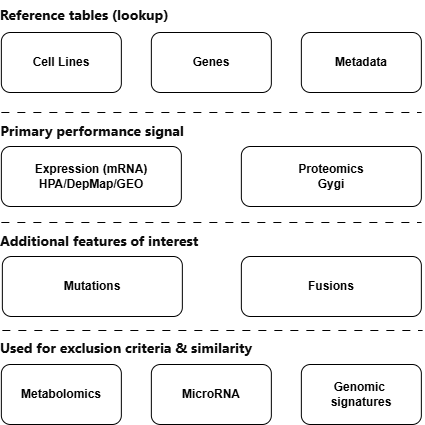
\includegraphics[width=0.55\textwidth]{figures/table_schema.png}
\caption{Data tables grouped by function: reference tables for lookup, expression and proteomics as primary performance measurements, mutations and fusions as additional features, and the remaining tables used for exclusion criteria and similarity.}
\label{fig:star-schema}
\end{figure}

Once the fourteen datasets had been collected and organised into the four categories described above, four main preprocessing challenges had to be resolved before the data could be used for ranking.

\begin{itemize}
  \item \textbf{Linking records across sources.} Each of the fourteen sources used its own identifier scheme for cell lines. A single shared identifier, DepMap's \texttt{ach\_id}, was adopted as the primary key used to join records across all sources.
  \item \textbf{Reconciling measurement units.} Expression values from DepMap were originally provided in log-transformed form, whereas expression values from other sources such as GEO and HPA were not. DepMap's expression values were converted back to linear-scale TPM before being combined with data from the other sources, so that all expression values were on a comparable scale.
  \item \textbf{Handling missing and invalid values.} Each dataset was checked for missing, null, and invalid entries (including N/A and infinite values), which were identified and cleaned. Duplicate records arising from overlapping calls across samples, such as repeated fusion events reported for the same cell line, were also identified and removed to ensure each event was represented once in the final table. This step was necessary to ensure that downstream ranking calculations, which depend on complete numerical inputs, were not skewed or broken by incomplete or duplicated records.
  \item \textbf{Restructuring from wide to long format.} The raw datasets were originally provided in wide format, with each cell line represented as a single row and each gene or feature as its own column. This format becomes impractical as the number of genes and features grows into the thousands, since filtering for a specific gene requires knowing its exact column name in advance, and joining wide tables requires matching potentially thousands of columns against one another. Figure~\ref{fig:wide-long} illustrates this transformation, using a small example.
\end{itemize}

\begin{figure}[h!]
\centering
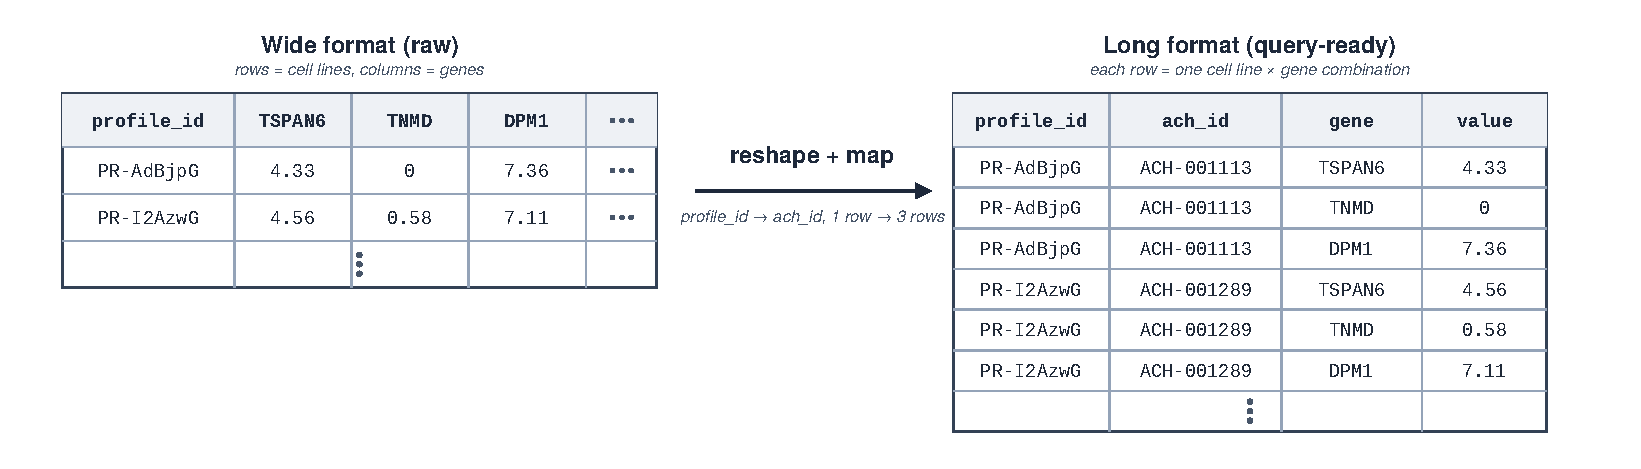
\includegraphics[width=\textwidth]{figures/wide_to_long.pdf}
\caption{Example transformation from wide format, with one row per
cell line and one column per gene, to long format, with one row per
cell line--gene combination. The \texttt{profile\_id} column carries
the raw identifier from the source file; \texttt{ach\_id} is resolved
via a separate profile-to-cell-line mapping before the data can be
joined with other harmonised sources.}
\label{fig:wide-long}
\end{figure}

The cleaned, long-format data was organised into the interlinked tables previewed in Figure~\ref{fig:star-schema}, distinguishing lookup tables, which store descriptive reference information about cell lines and genes, from measurement tables, which store the underlying multi-omics values one row at a time. The role of each group is as follows:

\begin{itemize}
  \item \textbf{Reference lookup tables} (cell lines, genes, metadata) hold no biological measurements themselves. They store descriptive attributes used to resolve identifiers and display results, and are joined against the measurement tables wherever a cell line or gene needs to be looked up by name.
  \item \textbf{Primary performance signal} (expression, proteomics) holds the core evidence used to compute a cell line's ranking score for a given target gene, combining transcript-level data from HPA, DepMap, and GEO with protein-level data from the Gygi lab.
  \item \textbf{Additional features of interest} (mutations, fusions) are not used to compute the ranking score itself, but support the include/exclude/ignore filtering described in Section~\ref{sec:celllinefinder-project}, allowing a query to be narrowed to cell lines with, or without, a specific genomic event.
  \item \textbf{Tables used for exclusion criteria and similarity} (metabolomics, microRNA, genomic signatures) are drawn on by the platform's exclusion filters and its similarity search feature, rather than contributing to the ranking score directly.
\end{itemize}

Beyond storing the raw values themselves, several measurement tables also carry annotation fields used elsewhere in the platform. The mutations table records, for each variant, flags indicating whether it is classified as a driver, a known hotspot, damaging, or loss-of-function; these annotations are surfaced directly to the user and are examined further in Section~\ref{sec::functional-testing}. The fusions table similarly records a confidence value and reading frame for each fusion event, used to indicate how strongly a given fusion call should be trusted.

The genomic signatures table is a partial exception to the wide-to-long restructuring described above: unlike the metabolomics and microRNA tables, it stores one row per cell line with a small, fixed set of columns (microsatellite instability, loss of heterozygosity, whole-genome doubling, chromosomal instability, ploidy, and aneuploidy) rather than one row per cell line--feature pair. This wide layout remains practical here because the number of signature types is small and fixed, unlike the thousands of genes or metabolites that motivated the restructuring of the other tables.

Table~\ref{tab:schema-tables} summarises the size and role of each table.

\begin{table}[h]
\centering
\begin{tabular}{|l|l|l|}
\hline
Table & Rows & Role \\
\hline
Cell line (lookup) & 2,220 & Reference info: growth pattern, doubling time \\
Gene (lookup) & $\sim$19,000 & Reference info: HUGO symbol, Entrez ID, chromosome \\
Metadata (lookup) & -- & Release version, harmonisation date, schema version \\
\hline
Expression & $\sim$20M & Primary signal: expression by source (DepMap/GEO/HPA) \\
Proteomics & $\sim$4.6M & Primary signal: protein intensity, detection flag \\
\hline
Mutations & $\sim$1M & Additional feature: driver/hotspot/damaging/LOF flags \\
Fusions & $\sim$190K & Additional feature: fusion events, confidence, frame \\
\hline
Metabolomics & $\sim$200K & Exclusion/similarity: cell line--metabolite levels \\
MicroRNA & $\sim$700K & Exclusion/similarity: cell line--miRNA levels \\
Genomic signatures & 1/cell line & Exclusion/similarity: MSI, LOH, WGD, CIN, ploidy \\
\hline
\end{tabular}
\caption{Summary of the interlinked tables in the final schema.}
\label{tab:schema-tables}
\end{table}

The table sizes reflect the underlying biology as much as the data engineering. Within the reference lookup tables, the gene table (\textasciitilde19,000 rows) is an order of magnitude larger than the cell line table (2,220 rows), simply reflecting that there are far more genes in the human genome than cell lines profiled by the platform's data sources.

The primary performance signal tables are by far the largest, since they store a value for every cell line--gene combination. Within this group, however, expression (\textasciitilde20M rows) substantially exceeds proteomics (\textasciitilde4.6M rows): transcriptomic profiling (microarray and RNA-seq) covers a much larger fraction of genes and cell lines than mass-spectrometry-based proteomics, which is technically more limited in coverage. This asymmetry is one reason a meaningful share of cell lines are annotated with an ``RNA only'' evidence scenario rather than ``RNA+Protein'', as seen in Section~\ref{sec::functional-testing}.

The additional feature tables are considerably smaller and differ from each other by an order of magnitude: mutations (\textasciitilde1M rows) substantially outnumber fusions (\textasciitilde190K rows), consistent with point mutations generally being a more frequent mode of genomic alteration than structural gene fusions.

A similar asymmetry appears among the tables used for exclusion criteria and similarity: microRNA (\textasciitilde700K rows) is around three times larger than metabolomics (\textasciitilde200K rows). The genomic signatures table is the smallest of all, at one row per cell line, since it stores a fixed set of summary scores per cell line rather than a value per cell line--feature pair.


% -----------------------------------------------------------------------------
\section{System Architecture}

\begin{figure}[h!]
    \centering
    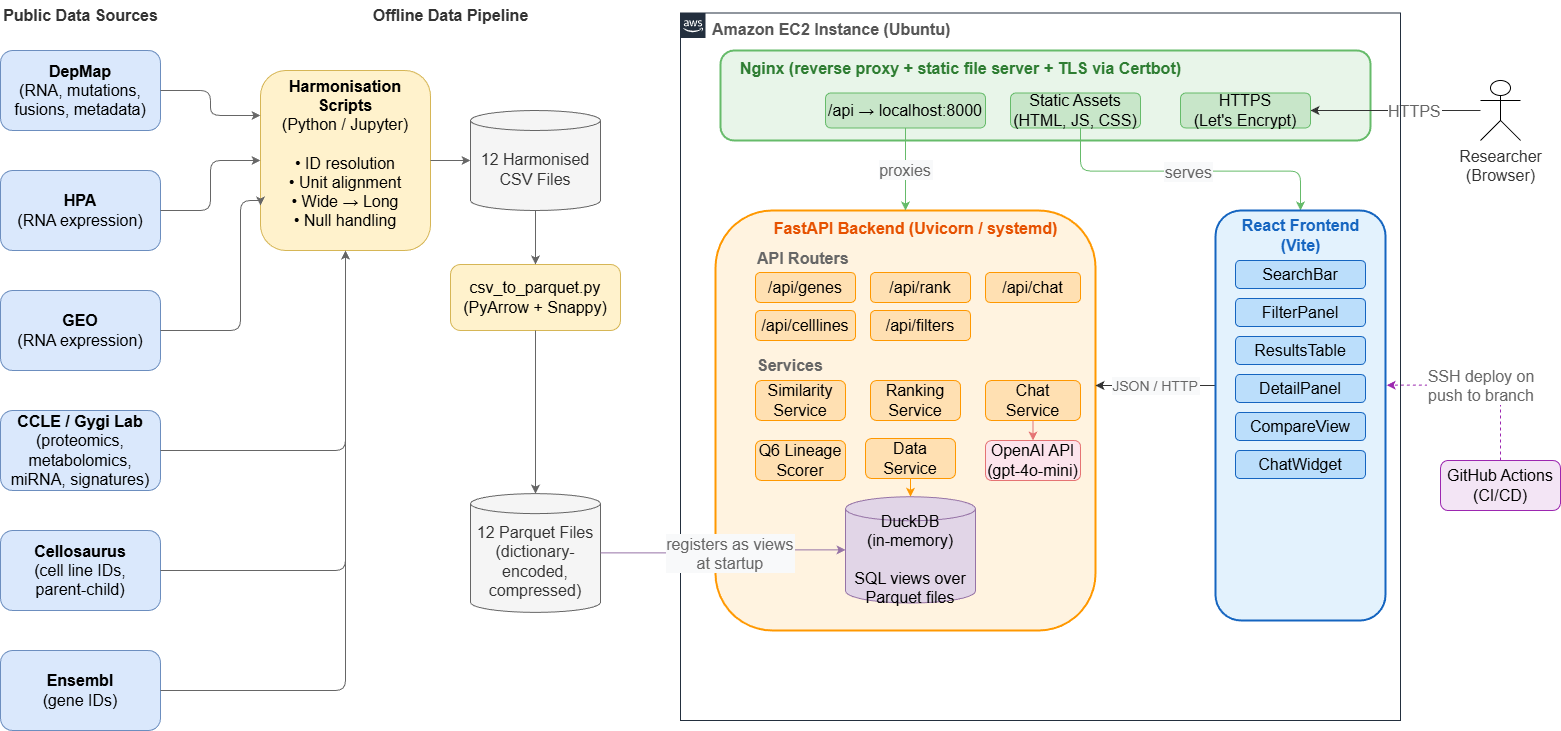
\includegraphics[width=\textwidth]{figures/system_architecture.drawio.png}
    \caption{High-level system architecture of CellLineFinder.}
    \label{fig:system-architecture}
\end{figure}

\subsection{Data Pipeline}
\label{sec:data-pipeline}
The fourteen datasets described in Section~\ref{sec:data-sources} pass through a three-stage offline pipeline. First, Python scripts clean each dataset: cell line names are resolved to DepMap accessions, gene symbols to Ensembl identifiers, DepMap's$\log_2(\text{TPM}+1)$ values are converted to linear TPM, and wide matrices are pivoted to long format keyed on \texttt{(ach\_id, ensembl\_id)}, producing eight harmonised CSVs. Second, a conversion script writes each CSV to Apache Parquet using PyArrow with Snappy compression and dictionary encoding, processing large tables in 500{,}000-row chunks. At startup the backend registers each Parquet file as a DuckDB view, so the data-access layer queries them via standard SQL.

\subsection{Backend API}
\label{sec:backend-api}
The backend is a Python web service built with FastAPI, exposing a stateless JSON API organised into four routers. The \textbf{gene router} (\texttt{/api/genes}) provides prefix-based autocomplete and symbol-to-Ensembl resolution. The \textbf{ranking router} (\texttt{/api/rank}) accepts a \textsc{POST} body specifying target genes with expression directions, weights, filter modes, exclusion criteria, and tissue preferences, delegates to the ranking service (Section~\ref{sec::ranking-algorithm}), and returns the ranked list. The \textbf{cell line router} (\texttt{/api/celllines}) serves an evidence-breakdown endpoint, a cosine-similarity endpoint (Section~\ref{sec:similarity}), and a side-by-side comparison endpoint. The \textbf{filter router} (\texttt{/api/filters}) returns the distinct disease, lineage, and subtype values with their valid pairings so the frontend can populate cascading dropdowns. All routers share a data-access layer that opens a new DuckDB cursor per request for thread safety. Pydantic schemas validate every request and response before computation.

\subsection{Frontend User Interface}
\label{sec:frontend-ui}

\begin{figure}[ht]
    \centering
    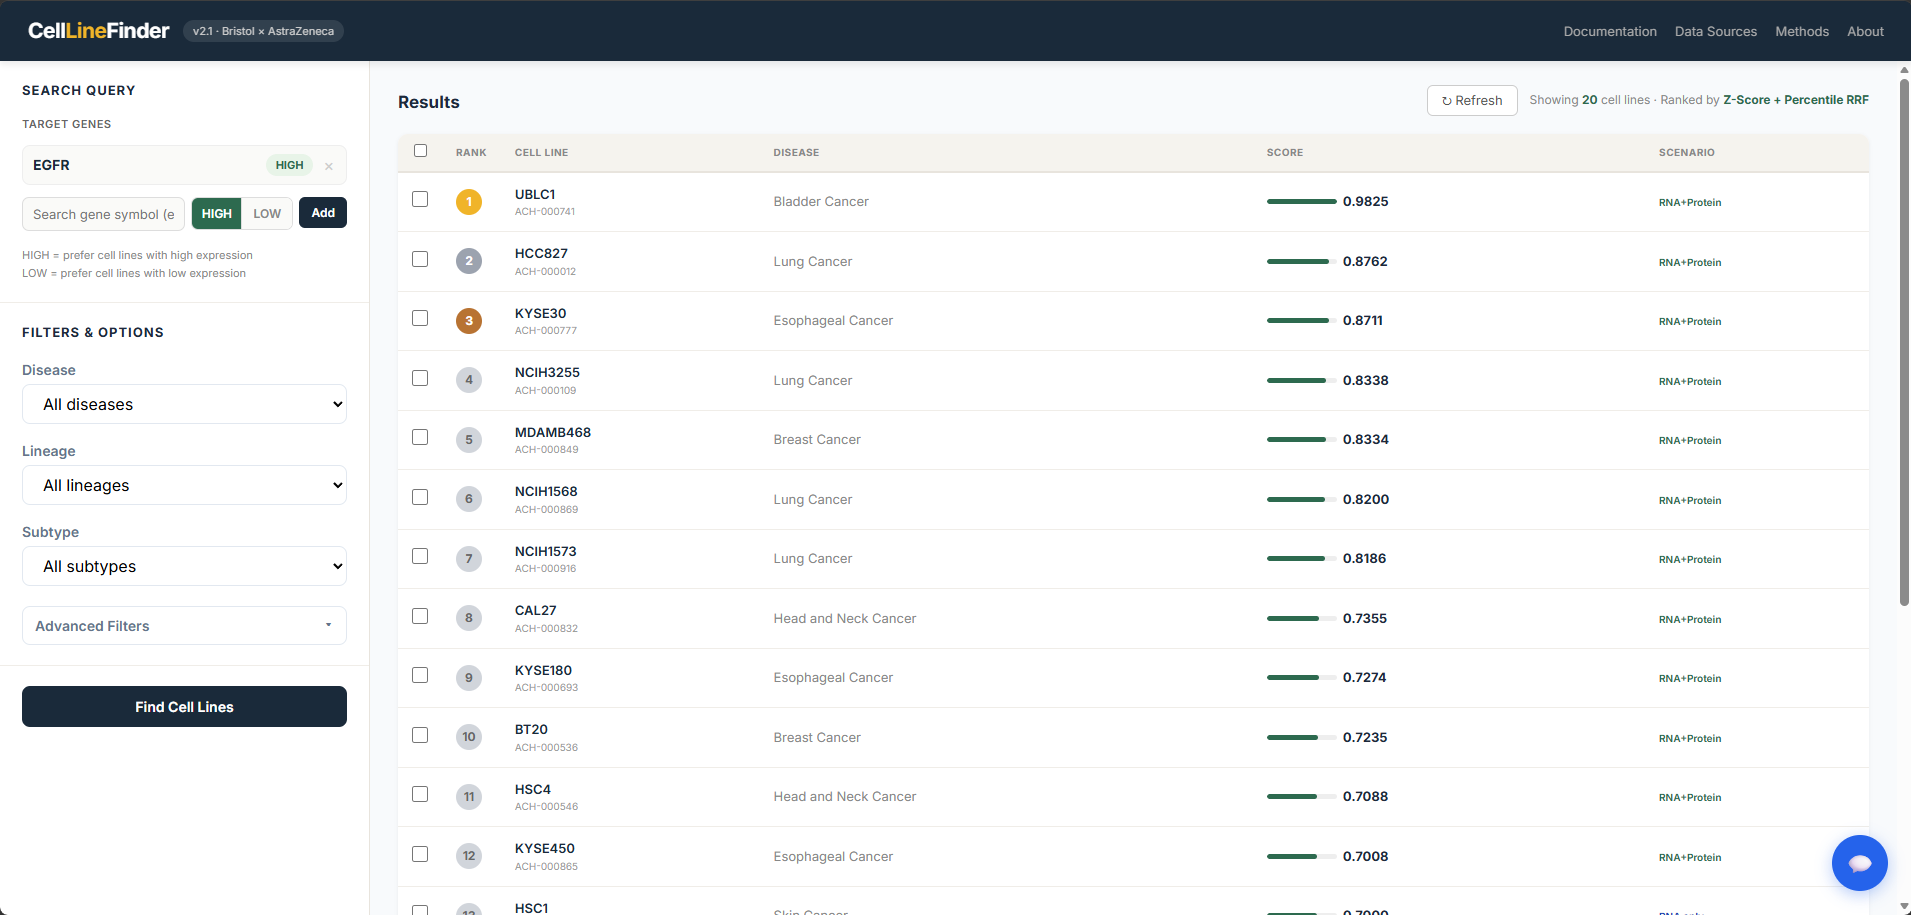
\includegraphics[width=\textwidth]{figures/frontend_ui}
    \caption{The CellLineFinder search interface showing ranked results for the EGFR gene target.}
    \label{fig:frontend-ui}
\end{figure}

The frontend is a single-page application built with React and bundled by Vite (Figure~\ref{fig:frontend-ui}). It communicates with the backend only through the JSON API described in Section~\ref{sec:backend-api}, and all rendering state is held in React hooks so that the interface updates without full page reloads. A \textbf{SearchBar} offers debounced autocomplete against the gene endpoint; each added gene carries a \textsc{high}/\textsc{low} toggle. The \textbf{FilterPanel} exposes cascading disease/lineage/subtype dropdowns, a hard-filter/soft-boost mode toggle, and an expandable advanced section for mutation/fusion modes, RNA-source toggles, an RNA:protein weight slider, instability thresholds, metabolite and miRNA exclusion, and a planned-assay selector, with a badge reporting how many advanced filters are active. The \textbf{ResultsTable} renders ranked results as a sortable table whose columns adapt to the active filters, and a CSV export button lets users download the current results with full query metadata for offline analysis. Selecting a row opens the \textbf{DetailPanel}, a slide-in overlay showing per-source scores, protein data, mutation and fusion annotations, and an on-demand list of the five most similar cell lines. Multiple rows can be compared side by side in the \textbf{CompareView} modal, with gene tabs for multi-gene queries. A \textbf{DocsModal} provides in-app documentation across four tabs covering usage, data sources, methodology, and project information.

\subsection{LLM-Powered Chatbot}
\label{sec::chatbot}
The ranking pipeline shown in Section~\ref{sec::ranking-algorithm} answers a single question. Given a target gene and a set of exclusion criteria, which cell lines rank highest? A researcher planning an experiment often has broader questions that sit alongside that ranking, such as which subtypes are represented in the catalogue, which lineages have data available for a given assay format, or what the recorded growth pattern of a returned cell line is. These are metadata queries rather than ranking queries, and a chatbot was added so the researcher can resolve them without leaving the results page. The chatbot is a function-calling loop built on the OpenAI Chat Completions API, using \texttt{gpt-4o-mini} by default and configurable through an environment variable. On each turn the model receives the conversation, a short system prompt describing its role, and the list of tools it may call. If it requests a tool, the backend runs it, appends the result, and returns the loop to the model. The loop is capped at five rounds per message, enough for common multi-step queries such as resolving a lineage and then searching within it, while preventing runaway calls when the question is misinterpreted. The system prompt tells the model to call a tool rather than answer from memory whenever the answer depends on project data, to quote the internal identifier of any cell line it mentions (for example \texttt{ACH-000012} for \texttt{HCC827}), and to decline questions outside the scope of cell line selection.

Five tools are exposed: \texttt{get\_gene\_context} returns AstraZeneca-curated notes for a small set of priority genes (FGFR2, CD86, ERBB2, KLK4, GAPDH, ASGR1, MUC1, CD3E). \texttt{search\_by\_lineage} returns the top five cell lines within a tissue lineage ranked by expression of a given gene, wrapping the main ranking. \texttt{lookup\_cell\_line} return metadata (disease, lineage, subtype, growth pattern) for a named cell line. \texttt{check\_assay\_compatibility} checks whether a cell line's growth pattern matches a planned assay format, reusing the profile definitions from Section~\ref{sec::assay-compat}, and \texttt{list\_options} returns the valid values for a category such as lineage or assay type, keeping the model within the vocabulary the other tools require for their exact-match lookups. Two design choices are worth noting. Function calling was preferred over retrieval-augmented generation because the underlying data is structured records where exact identifiers and numeric values matter, and delegating each lookup to the same SQL used by the ranked table means the chatbot cannot drift from the source of truth. \texttt{gpt-4o-mini} was chosen over larger models because the operation the chatbot performs sit within it capability, while one-to-two second response time is faster inside a workflow that already involves waiting for the ranking pipeline. The chatbot does not replace the pipeline. It sits alongside it and anything that requires combining evidence across many cell lines is still routed through the ranking service.

\subsection{Deployment}
The application is deployed on one Amazon EC2 instance: the backend is a \texttt{systemd} service running Uvicorn, and Nginx serves the compiled frontend as static assets, reverse-proxying \texttt{/api} requests to the local loopback interface. HTTPS is provided by Certbot (Let's Encrypt). A GitHub Actions workflow runs on every push to \texttt{mew/ranking-v2} and connects over SSH, pulls the latest code, rebuilds dependencies, restarts the service and runs a health-check against \texttt{/health} so a merged change is live within minutes.

% -----------------------------------------------------------------------------
\section{Ranking Algorithm}
\label{sec::ranking-algorithm}
\subsection{Multi-Omics Data Weighting}
\label{sec:weighting}
\noindent
\textbf{Cell line ranking score (single gene).}
The steps below describe scoring for a single gene. Multi-gene queries build on this by fusing the per-gene ranks produced
here.

\noindent
The algorithm scores cell lines for a gene in four steps:

\begin{enumerate}
    \item Rank cell lines within each RNA source (DepMap, HPA, GEO) by
          z-score and by percentile.
    \item Fuse these per-source ranks into a single RNA score via
          \emph{averaged} Reciprocal Rank Fusion (RRF).
    \item Repeat steps 1--2 for protein intensity (one source only, so
          two rank lists rather than six).
    \item Normalise the RNA and protein RRF scores to $[0,1]$ and
          combine them with weights $w_{\text{rna}}, w_{\text{protein}}$
          into the cell line's \texttt{combined\_score}.
\end{enumerate}

\paragraph{Step 1: per-source ranking.}
Within each source, a cell line's expression value $x$ for the gene is
converted into two rankings. The \emph{z-score}
\begin{equation}
z = \frac{x - \mu}{\sigma}
\label{eq:zscore}
\end{equation}
standardises $x$ against the source's mean $\mu$ and standard deviation
$\sigma$; cell lines are ranked in descending order of $z$. The
\emph{percentile rank}
\begin{equation}
p = \frac{\#\{x_i \le x\}}{n}
\label{eq:percentile}
\end{equation}
gives the proportion of the $n$ cell lines in that source at or below
$x$, again ranked descending. The two measures are kept separate
because they are sensitive to different failure modes: the z-score
captures the magnitude of an outlier, while the percentile rank is
robust to it, being unaffected by how large the gap to the next value
is. Requiring a cell line to score well under both reduces the risk of
a single extreme value in one source dominating the result.

\paragraph{Step 2: fusing ranks via RRF.}
Each rank $r$ is converted to a score
\begin{equation}
\text{RRF}(r) = \frac{1}{k + r}
\label{eq:rrf}
\end{equation}
where $k$ is a smoothing constant that dampens the influence of very
low ranks. We follow the original RRF formulation and set $k=60$, the
value found to perform best on average across TREC benchmarks in the
original study~\cite{cormack2009} and widely adopted as the
default in subsequent applications of RRF.

Up to six rank lists (three sources $\times$ two methods) are then
fused per cell line by \emph{averaging} rather than summing:
\begin{equation}
\text{score}_i = \frac{1}{N_i} \sum_{j=1}^{N_i} \text{RRF}(r_{ij})
\label{eq:rrf-avg}
\end{equation}
where $N_i$ is the number of rank lists that actually cover cell line
$i$. Averaging (instead of a raw sum) prevents cell lines missing a
data source from being penalised relative to those with full
coverage: a cell line ranked highly in two of three sources is judged
on those two ranks alone, not pushed down for lacking a third. Source
coverage is tracked separately and can be filtered on explicitly,
rather than being baked into the score.

\paragraph{Step 3: protein ranking.}
Protein intensity is ranked identically (Equations~\ref{eq:zscore}--\ref{eq:rrf-avg}),
fusing two rank lists (z-score, percentile) rather than six, since
protein data comes from a single source.

\paragraph{Step 4: combining into a final score.}
The fused RNA and protein RRF scores are each min-max normalised to
$[0,1]$ -- necessary since they are not directly comparable in raw
form, being derived from different numbers of rank lists -- then
combined as
\begin{equation}
\text{combined\_score} = w_{\text{rna}} \cdot \text{expr}_{\text{norm}} + w_{\text{protein}} \cdot \text{protein}_{\text{norm}}
\label{eq:final-score}
\end{equation}
with defaults $w_{\text{rna}}=0.7$, $w_{\text{protein}}=0.3$. Depending
on data availability, a cell line falls into one of four scenarios:
both terms contribute (\emph{RNA+Protein}); only the RNA term
(\emph{RNA only}); only the protein term (\emph{Protein only}); or, if
neither modality has data for the gene, the cell line is excluded.

\paragraph{From score to rank.}
Cell lines are finally ordered by \texttt{combined\_score} according to
the gene's queried direction. For a \emph{high}-expression query, cell
lines are sorted in descending order of \texttt{combined\_score} so
that the highest-scoring cell line receives rank 1. For a
\emph{low}-expression query, the sort order is reversed, so that the
lowest-scoring cell line receives rank 1. This per-gene rank is the
quantity fused across genes when multiple genes are queried together,
described next. In the deployed interface this value is shown simply
as \textbf{\textit{Score}}, without the underlying field name.

\paragraph{Worked example.}
Table~\ref{tab:worked-example} traces the pipeline end to end for a
\emph{high}-expression query on EGFR, cell line UBLC1 (ACH-000741).
UBLC1 has expression data in two of the three RNA sources (DepMap and
HPA, but GEO has no recorded value for this cell line) and is present in
the protein dataset.

\begin{table}[h!]
\centering
\caption{Per-source values and ranks for EGFR, cell line UBLC1.}
\label{tab:worked-example}
\begin{tabular}{lccccc}
\hline
\textbf{Source} & \textbf{Value} & \textbf{Z-score} & \textbf{Percentile} & \textbf{Z-rank} & \textbf{Pct-rank} \\
\hline
DepMap & TPM 1078.5 & +14.12 & 99.9\% & 2 & 2 \\
HPA & TPM 906.2 & +8.58 & 99.8\% & 3 & 3 \\
GEO & no data & -- & -- & -- & -- \\
Protein (Gygi) & Intensity 5.15 & +3.27 & 100\% & 1 & 1 \\
\hline
\end{tabular}
\end{table}

Following Equation~\ref{eq:rrf-avg}, the four RNA rank lists (DepMap
and HPA, z-score and percentile each) fuse with $N_i=4$, since GEO
does not cover this cell line:
\[
\text{expr\_rrf} = \tfrac{1}{4}\left(\tfrac{1}{62}+\tfrac{1}{62}+\tfrac{1}{63}+\tfrac{1}{63}\right) \approx 0.0160.
\]
The two protein rank lists fuse identically with $N_i=2$:
\[
\text{prot\_rrf} = \tfrac{1}{2}\left(\tfrac{1}{61}+\tfrac{1}{61}\right) \approx 0.0164.
\]
Min-max normalising against all other cell lines scored for EGFR
gives $\text{expr}_{\text{norm}} \approx 0.975$ and
$\text{protein}_{\text{norm}} = 1.000$ (UBLC1 holds the single highest
protein rank for EGFR, so it receives the maximum normalised protein
score). Both modalities are available, so Equation~\ref{eq:final-score}
with the default weights gives
\[
\text{combined\_score} = 0.7(0.975) + 0.3(1.000) = 0.9825,
\]
matching the score returned by the deployed system under the
\emph{RNA+Protein} scenario, which ranks UBLC1 first among all cell
lines for this query.


\paragraph{Cell line ranking score (multiple genes).}
When more than one gene is queried, each gene is first ranked
independently as described above, producing a per-gene rank for every
cell line. These per-gene ranks are then fused into a single overall
ranking in two steps.

\paragraph{Step 5: fusing per-gene ranks.}
For a query over genes $g = 1, \ldots, m$, let $\text{rank}_i^{(g)}$
denote cell line $i$'s per-gene rank from gene $g$'s pipeline. These
ranks are fused via the same RRF formula as before (Equation~\ref{eq:rrf}),
summed across genes rather than averaged, and rescaled to $[0,1]$:
\begin{equation}
\text{final\_score}_i = \frac{1}{S_{\max}} \sum_{g=1}^{m} \text{RRF}\left(\text{rank}_i^{(g)}\right),
\qquad S_{\max} = \frac{m}{k+1}
\label{eq:multi-rrf}
\end{equation}
$S_{\max}$ is the value the sum would take if cell line $i$ held rank
1 in every one of the $m$ queried genes simultaneously. Unlike the
per-source fusion in Step 2, contributions here are \emph{summed}
rather than averaged, so a cell line ranked highly across more genes
accumulates a correspondingly higher score. Because $S_{\max}$ is a
fixed theoretical ceiling rather than the maximum score actually
achieved within the query result, a score of 1.0 is reached only by a
cell line ranking first in every queried gene at once; the top-ranked
cell line overall will generally score slightly below 1.0. If a cell
line has no per-gene rank for a given gene (because it had neither
RNA nor protein data for that gene, see Step 4), that gene
contributes no term to the sum for that cell line.

Because each gene's direction (\emph{high} or \emph{low}) is already
resolved into its per-gene rank -- rank 1 always denotes the most
desirable cell line for that gene, regardless of direction -- cell
lines are ordered by $\text{final\_score}_i$ in descending order
irrespective of the directions queried for the individual genes.

\paragraph{Step 6: merging coverage confidence.}
Each cell line's overall coverage confidence is taken as the mean of
its per-gene coverage-confidence values (Step 4) across the genes for
which it has a rank. As this per-gene value takes only the discrete
values $1.0$, $w_{\text{rna}}$, or $w_{\text{protein}}$, a cell line
lacking full RNA and protein coverage in any one queried gene pulls
down its averaged confidence across the whole query.

\paragraph{Worked example (continued).}
Continuing the previous example with both genes queried together
(\emph{high}): UBLC1 ranks \#1 among cell lines scored for EGFR and
\#2 for SEC61G. From Equation~\ref{eq:rrf},
\[
\text{RRF}(1) = \tfrac{1}{61} \approx 0.016393, \qquad
\text{RRF}(2) = \tfrac{1}{62} \approx 0.016129,
\]
giving a raw sum of $0.032523$. With $m=2$ genes,
$S_{\max} = 2/61 \approx 0.032787$, so
\[
\text{final\_score} = 0.032523 / 0.032787 \approx 0.9919,
\]
matching the score shown by the deployed system. UBLC1 falls just
short of 1.0 because it does not hold rank 1 in \emph{both} queried
genes, even though it remains the top-ranked cell line overall.


\subsection{Confidence Score Design}
\label{sec:confidence-score}
\noindent
\noindent\textbf{Confidence score design.}
We refer to \texttt{combined\_score} (Equation~\ref{eq:final-score}) as
a \emph{confidence score}, since each step in its construction
requires independent evidence to agree before contributing to a high
value: within-source agreement between z-score and percentile
(Step 1), cross-source agreement via averaged RRF (Steps 2--3), and
cross-modality agreement between RNA and protein (Step 4). A cell
line only receives a high score when several independent lines of
evidence point the same way, rather than any single measurement.

\noindent\textbf{Trade-offs.}
This design has several limitations. The confidence score is ordinal,
not probabilistic: it supports relative comparisons between cell
lines rather than an absolute measure such as a confidence interval.
Because RRF averages rather than sums, coverage is not penalised
directly, so a cell line with data from two sources can score
identically to one with all three, provided its ranks are equally
strong. RRF also discards the magnitude of differences between cell
lines, retaining only relative rank. Finally, the weights
$w_{\text{rna}}=0.7$ and $w_{\text{protein}}=0.3$ are heuristic rather
than empirically validated, and since they are user-adjustable, the
score's meaning is not fixed across sessions.

\subsection{Mutation Filtering}
\label{sec:mutation-filter}
\noindent
Mutation status is categorical: a cell line either carries a given
mutation or it does not, determined from DepMap's somatic mutation
profiles. The pipeline supports an optional hard filter on this
status, applied after the confidence score is computed, with three
modes: \emph{ignore} (no filtering), \emph{include} (keep only cell
lines with a recorded mutation in the gene), and \emph{exclude}
(remove them). It is a hard filter rather than a weighting term
because mutation status cannot be meaningfully combined with a
continuous expression-based score, and this separation lets users
apply it selectively without changing how confidence is scored for
the cell lines that remain.

For a cell line that passes this filter, the platform surfaces the
variant, its type, predicted protein effect, four boolean flags
(driver, hotspot, damaging, loss of function), and the percentage of
reads supporting the call. These are shown for context only and play
no part in the include/exclude logic itself. A worked example of this
annotation, for cell line HCC827, is given in
Table~\ref{tab:egfr-mutation-detail} in Section~4.2.

\subsection{Fusion Filtering}
\label{sec:fusion-filter}
\noindent
A gene fusion joins parts of two separate genes into a hybrid
transcript, typically through a chromosomal rearrangement, and is
therefore indexed by a pair of genes rather than a single one. As
with mutation status, a parallel hard filter is available, applied
after the confidence score is computed, with the same three modes:
\emph{ignore} (no filtering), \emph{include} (keep only cell lines
with a recorded fusion involving the gene, from DepMap's fusion event
data, matched by gene symbol), and \emph{exclude} (remove them).

For a cell line with a recorded fusion, the platform surfaces the
fusion name (\texttt{GENE1--GENE2}), a confidence label, the reading
frame (\emph{in-frame} or \emph{out-of-frame}, which affects whether
a functional fusion protein is likely produced), and fusion fragments
per million reads. As with mutation annotations, these are shown for
context only and play no part in the include/exclude logic. A worked
example of this annotation, for cell line UBLC1, is given in
Table~\ref{tab:ublc1-fusion-detail} in Section~4.2.

Mutation and fusion filters are independent, so a user may apply
either in isolation or combine them, for example excluding mutated
cell lines while including only those with a specific fusion. Both
are applied after the confidence score is computed, so a cell line's
score is unaffected by whether it is subsequently included in or
excluded from the results.

\subsection{Disease Indication}
\label{sec::disease-indication}

The ranking components described so far judge each cell line on the strength of its molecular evidence for a target gene, but they do not know what tissue the user is interested in. A researcher planning a lung cancer experiment and one planning a bladder cancer experiment can send the same target gene and receive the same ordered list, because the RNA and protein scores are computed across the whole cell line universe. The disease indication component address this by taking three optional inputs \texttt{target\_lineage}, \texttt{target\_disease}, and \texttt{target\_subtype}, and using them to reshape the ranking without discarding cell lines from outside the requested tissue.

Each cell line is assigned a match score $q_6$ under a four-tier hierarchy, evaluated in the order below and taking the first tier that applies:

\begin{itemize}
    \item \textit{Exact subtype}($q_6 = 1.0$): the cell line's subtype matches \texttt{target\_subtype} and if a lineage is also specified, its lineage matches \texttt{target\_lineage}. The joint check prevents cross-tissue false positives when a subtype label such as "Adenocarcinoma" occurs in several unrelated tissues. 
    \item \textit{Same disease}($q_6 = 0.75$): the cell line's primary disease matches \texttt{target\_disease}.
    \item \textit{Same lineage}($q_6 = 0.5$): the cell line's lineage matches \texttt{target\_lineage}. 
    \item \textit{No match}($q_6 = 0$): none of the above applies. 
\end{itemize}

The confidence score defined in Equation~\ref{eq:q6-boost} is then adjusted by a soft-boost multiplier:
\begin{equation}
    \text{score}_{\text{final}} = \text{score}_{\text{base}} \times (0.7 + 0.3 \cdot q_6)
    \label{eq:q6-boost}
\end{equation}

An exact subtype match leaves the base score unchanged, a disease match retains 92.5\%, a lineage match 85\%, and an unrelated cell line 70\%. The multiplier is applied after upstream ranking and filtering, so the base score is preserved and reported alongside the adjusted final score. Table~\ref{tab:q6-hierarchy} shows the four tiers on concrete query.

\begin{table}[h]
\centering
\begin{tabular}{|l|l|l|l|l|c|c|}
\hline
Cell line & Lineage & Primary disease & Subtype & Match level & $q_6$ & Multiplier \\
\hline
HCC827   & lung          & Lung Cancer   & NSCLC Adenocarcinoma        & exact\_subtype & 1.00 & 1.000 \\
NCIH1341 & lung          & Lung Cancer   & SCLC                        & same\_disease  & 0.75 & 0.925 \\
SALE     & lung          & Non-Cancerous & --                          & same\_lineage  & 0.50 & 0.850 \\
UBLC1    & urinary\_tract & Bladder Cancer & Transitional Cell Carcinoma & none          & 0.00 & 0.700 \\
\hline
\end{tabular}
\caption{Disease indication annotation example. Query target: \texttt{target\_lineage}~=~\emph{lung}, \texttt{target\_disease}~=~\emph{Lung Cancer}, \texttt{target\_subtype}~=~\emph{Non-Small Cell Lung Cancer (NSCLC), Adenocarcinoma}. Each cell line receives a match level and multiplier under Equation~\ref{eq:q6-boost}, applied to its base confidence score.}
\label{tab:q6-hierarchy}
\end{table}

A hard filter on lineage or disease is still available though \texttt{disease\_filter} and \texttt{lineage\_filter}. When selecting, it will removes cell lines that may still be scientifically relevant. For example, a related-tissue line that expresses the target more strongly than any line from the requested tissue. The soft-boost formulation keeps such cell lines visible while ensuring that a well-matched cell line within the requested tissue outranks an unmatched line of comparable base score. 

The boost is intentionally bounded. A cell line from the requested tissue with a very low base score cannot climb the ranking on tissue match alone, and when the target gene is barely expressed in the requested tissue, the top of the ranked list may contain no matching cell lines. In that case the returned $q_6$ values and match labels make the absence visible rather than concealing it behind a filter that would have returned nothing.


\subsection{Exclusion Criteria}
\label{sec:exclusion}

Exclusion criteria let a scientist rule out a cell line on grounds unrelated to the target gene. Four are implemented: microsatellite instability and chromosomal instability from the genomic signatures table, the level of a named metabolite, and the expression of a named miRNA. Each is set as a threshold on the ranking endpoint, and each removes cell lines whose measured value is above it.

These criteria differ from the rest of the pipeline in what they describe. Expression, protein, and mutation evidence all answer a question about the target gene in a given cell line. Instability, metabolic state and miRNA expression describe the cell line itself, regardless of the gene being studied. So, they are applied as removals rather than folded into the score.

Exclusion is a hard removal rather than a score penalty because it expresses a constraint, not a preference. A scientist ruling out an unstable line is not saying that line is worse; they are saying it is unusable for the experiment they intend to run. A penalty would allow such a line to reach the top of a sparse result set, which is precisely the case where the exclusion matters most.

No criterion has a default threshold. Both the measure and the cut-off must be supplied, and a request giving one without the other is rejected rather than silently ignored. The reason is visible in the data: lactate levels across 928 cell lines range from 4.11 to 6.63 with a standard deviation of 0.27, while hsa-miR-21 across 952 cell lines ranges from 14.5 to 188,089 with a standard deviation of 9,810. The two are on incomparable scales, and no single default could be meaningful for both. More importantly, the tool has no basis to determine which lactate level disqualifies a cell line. That decision belongs to the scientist, and inventing one would produce exclusions difficult to explain.

Missing measurements do not exclude. The filters remove cell lines known to exceed the threshold, so a line with no recorded MSI value is retained rather than discarded. Coverage makes this necessary: only 365 of the 1,581 ranked cell lines have mutation data, and the signature, metabolomic and miRNA tables each cover a different subset. Treating absence as failure would remove most of the ranking for reasons that have nothing to do with biology.

\subsection{Similarity Component}
\label{sec:similarity}

The highest-ranked cell line is not always the one a scientist can use. It may be unavailable, slow to culture, or unsuited to the intended assay, and a result resting on a single line is fragile. The similarity component answers a different question from the ranking: not which cell lines express the target, but which cell lines resemble a chosen one.

Resemblance is measured over the 2,000 genes with the highest variance in DepMap expression, selected from 53,538. Restricting the feature space is necessary because distances concentrate as dimensionality grows, so a comparison across every gene is dominated by genes that do not distinguish cell lines at all. Variance is computed on $\log_2(\text{TPM}+1)$ rather than on raw values, and the distinction is not cosmetic. Raw variance is dominated by genes that are simply highly expressed rather than by genes that vary between cell lines, so the two criteria select different sets: only 712 of the 2,000 genes overlap. An early version of the service selected on raw values while the validated notebook used log values, which meant that just over a third of the intended gene set was in use.

Missing values are filled with the column median, and each feature is then z-scored across cell lines. Table~\ref{tab:layer-separation} shows why this matters. On 114 same-lineage pairs against 1,886 different-lineage pairs, raw cosine similarity separates lineages by 0.105, while the same comparison on z-scored features separates them by 0.307. Scaling nearly triples the separation the method exists to produce, because without it a handful of high-magnitude genes dominate every comparison. Repeating the test across five random samples gave gaps between 0.264 and 0.325, so the figure is not an artefact of one sample.

Similarity between two cell lines is the cosine of the angle between their scaled expression vectors. Cosine was chosen over Euclidean distance because it compares the shape of an expression profile rather than its overall magnitude, so two lines with the same relative pattern are judged similar even when one is globally more transcriptionally active.

The reported score combines expression with proteomics where both cell lines carry it. The two are not comparable in raw form: across the 369 cell lines with both layers, expression similarity has a standard deviation of 0.181 and protein similarity 0.118, so an unadjusted protein contribution would be systematically smaller simply because its values are less spread out. Protein similarity is therefore rescaled by the ratio of the two spreads before weights of 0.7 and 0.3 are applied. Where a pair shares only expression, the score is the expression similarity alone rather than a penalised combination. This follows the same reasoning as the averaged rank fusion in Section~\ref{sec:weighting}: a cell line is judged on the evidence available for it, not on how much evidence exists.

Metabolomics, miRNA and genomic signatures are reported alongside each result but do not contribute to the score. The three were tested as a combined feature space of 965 features across the 895 cell lines carrying all of them, and separated lineages by 0.080 against expression's 0.307. Across five samples that figure ranged from 0.055 to 0.080. Genomic signatures were dropped from the score entirely: six dimensions are too few for a stable cosine, and across all 1,910,035 cell line pairs, 16.3\% score above 0.8 and 34.1\% above 0.5. A high signature similarity therefore carries almost no information about whether two lines are alike. The same table still drives the exclusion criteria in Section~\ref{sec:exclusion}, where a threshold on one named measure does not require a stable distance.

Results are flagged for derivation. Cell lines derived from one another share an origin rather than corroborating a finding independently, and a derivative scores highly on similarity for exactly that reason. Relationships form chains, so each cell line is resolved to the root it descends from and two lines are flagged as related when their roots agree. Coverage is limited: only 86 of the 2,220 cell lines have a parent recorded, so the flag identifies known derivatives rather than guaranteeing independence.

Separation is strongly lineage-dependent. Haematological lineages separate cleanly, with lymphocyte and blood showing gaps of 0.659 and 0.601, while lung is weakest at 0.081 across 210 lines. Validation on HCC827, itself a lung line, nonetheless returns ten NSCLC lines out of ten, with its derivative HCC827GR5 ranked first and marked as such: correct as a similarity result, and useless as an independent alternative, which is the distinction the flag exists to make.

\begin{table}[!htbp]
\centering
\caption{Mean cosine similarity within and between lineages, before and after
scaling.}
\label{tab:layer-separation}
\begin{tabular}{lrrr}
\hline
\textbf{Feature set} & \textbf{Same} & \textbf{Different} & \textbf{Gap} \\
\hline
Expression, raw       & 0.785 & 0.680    & +0.105 \\
Expression, z-scored  & 0.287 & $-$0.020 & +0.307 \\
Contextual, raw       & 0.633 & 0.572    & +0.062 \\
Contextual, z-scored  & 0.080 & $-$0.001 & +0.080 \\
\hline
\end{tabular}
\end{table}


\subsection{Assay Compatibility}
\label{sec::assay-compat}

Even a cell line with strong molecular evidence for the target gene is only useful in practice if it can be grown in the format the planned experiment needs. Since adherent cells cannot be used in a suspension screen and vice versa, the compatibility check is surfaced as a per-cell annotation rather than folded into the score.

When the user supplies an \texttt{assay\_type} parameter, each cell line receives one of two labels.

\begin{itemize}
    \item \textbf{OK}: the cell line's recorded growth pattern is in the set allowed for the requested assay. No warning shown.
    \item \textbf{WARN}: the cell line either has no growth pattern on record, or its growth pattern is outside the allowed set. A short reason is attached, for example \emph{"growth pattern unknown"} or \emph{"growth is 2D: suspension (need 2D: adherent)"}.
\end{itemize}

Four assay profiles are exposed: \texttt{adherent\_screen} and \texttt{3d\_spheroid} both require \texttt{2D: adherent}, \texttt{suspension\_screen} requires \texttt{2D: suspension}, and \texttt{flexible} accepts any of the three growth patterns. Adding a new assay requires only a new entry in the profile file.

The check does not remove any cell line from the ranking. A hard filter was considered but rejected because the growth pattern field is often missing. 1,158 of the 2,220 cell lines in the dimension table (52\%) are recorded as \texttt{unknown}, and dropping all of them would strip most of the ranked list without scientific reason. The annotation is applied after all upstream ranking and filtering, so the OK/WARN label carries no weight in the ranking.

In summary, the pipeline described throughout this section
is set out as pseudocode in Algorithms~\ref{alg:run-ranking}
and~\ref{alg:similarity}: the former covering gene-based ranking
together with its filters, exclusions, and annotations, and the
latter covering similarity ranking between cell lines.

\bigskip

\begin{algorithm}[H]
\caption{Cell line ranking pipeline for a set of query genes}
\label{alg:run-ranking}
\KwIn{Genes $G$ (direction \emph{high}/\emph{low} each), weights $w_{\text{rna}}, w_{\text{protein}}$, mutation/fusion modes, exclusion thresholds, disease-indication targets, assay type}
\KwOut{Ranked cell lines with final score, confidence, and annotations}
\ForEach{gene $g \in G$}{
    $\text{expr\_rrf}_g \gets$ RankExpression($g$)\;
    $\text{prot\_rrf}_g \gets$ RankProtein($g$)\;
    $\text{combined}_g \gets$ CombineRnaProtein($\text{expr\_rrf}_g$, $\text{prot\_rrf}_g$, $w_{\text{rna}}$, $w_{\text{protein}}$)\;
    $\text{combined}_g \gets$ ApplyMutationFilter($\text{combined}_g$)\;
    $\text{combined}_g \gets$ ApplyFusionFilter($\text{combined}_g$)\;
}
\eIf{$|G| = 1$}{
    $\text{final} \gets$ SortByScore($\text{combined}_{g_1}$, direction of $g_1$)\;
}{
    \ForEach{gene $g \in G$}{
        $\text{rank}_g \gets$ RankByScore($\text{combined}_g$, direction of $g$)\;
    }
    $\text{final.score} \gets$ FuseRanksRRF($\{\text{rank}_g\}$, average $=$ False) $/ S_{\max}$\;
    $\text{final.confidence} \gets$ mean of per-gene coverage confidences\;
}
$\text{final} \gets$ ApplyExclusionCriteria($\text{final}$)\;
\If{disease-indication targets supplied}{
    $\text{final.score} \gets \text{final.score} \times (0.7 + 0.3\, q_6)$\;
    Re-sort $\text{final}$ by boosted score\;
}
\If{assay type supplied}{
    Annotate $\text{final}$ with OK/WARN (does not reorder)\;
}
\Return{$\text{final}$}
\end{algorithm}


\bigskip


\begin{algorithm}[H]
\caption{Similarity ranking for a query cell line}
\label{alg:similarity}
\KwIn{Query cell line $q$, expression matrix (top 2{,}000 log-variance genes), protein similarity data, derivative/ancestry table}
\KwOut{Ranked candidate cell lines with similarity score and derivative flag}
$X \gets$ SelectTopVarianceGenes($\log_2(\text{TPM}+1)$, $n=2000$)\;
$X \gets$ ImputeMissing($X$, method $=$ median)\;
$X \gets$ ZScore($X$, per gene across cell lines)\;
\ForEach{candidate cell line $c \ne q$}{
    $\text{sim}_{\text{expr}} \gets$ CosineSimilarity($X_q$, $X_c$)\;
    \eIf{both $q$ and $c$ have protein data}{
        $\text{sim}_{\text{prot}} \gets$ CosineSimilarity(protein$_q$, protein$_c$) $\times \sigma_{\text{expr}} / \sigma_{\text{prot}}$\;
        $\text{score}_c \gets 0.7\,\text{sim}_{\text{expr}} + 0.3\,\text{sim}_{\text{prot}}$\;
    }{
        $\text{score}_c \gets \text{sim}_{\text{expr}}$\;
    }
    $\text{is\_derivative}_c \gets$ [Root($q$) $=$ Root($c$)]\;
}
\Return{candidates sorted by $\text{score}$ descending, flagged for derivation}
\end{algorithm}

% -----------------------------------------------------------------------------

% -----------------------------------------------------------------------------

% -----------------------------------------------------------------------------



% {\bf A topic-specific chapter, roughly 30\% of the total page-count}
% \vspace{1cm} 

% \noindent
% This chapter is intended to describe what you did: the goal is to explain
% the main activity or activities, of any type, which constituted your work 
% during the project.  The content is highly topic-specific. For some 
% projects it will make sense to split the content into two main sections, or maybe even into two separate chapters: one 
% will discuss the design of something, including any rationale or decisions made, 
% and the other will discuss how this design was realised via some form of 
% implementation.  You could instead give this chapter the title ``Design and Implementation"; or you might split this content into two chapters, one titled ``Design" and the other ``Implementation" .

% Note that it is common to include evidence of ``best practice'' project 
% management (e.g., use of version control, choice of programming language 
% and so on).  Rather than simply a rote list, make sure any such content 
% is useful and/or informative in some way: for example, if there was a 
% decision to be made then explain the trade-offs and implications 
% involved.

% \section{Example Section}

% This is an example section; 
% the following content is auto-generated dummy text.
% \lipsum

% \subsection{Example Sub-section}

% \begin{figure}[t]
% \centering
% foo
% \caption{This is an example figure.}
% \label{fig}
% \end{figure}

% \begin{table}[t]
% \centering
% \begin{tabular}{|cc|c|}
% \hline
% foo      & bar      & baz      \\
% \hline
% $0     $ & $0     $ & $0     $ \\
% $1     $ & $1     $ & $1     $ \\
% $\vdots$ & $\vdots$ & $\vdots$ \\
% $9     $ & $9     $ & $9     $ \\
% \hline
% \end{tabular}
% \caption{This is an example table.}
% \label{tab}
% \end{table}

% \begin{algorithm}[t]
% \For{$i=0$ {\bf upto} $n$}{
%   $t_i \leftarrow 0$\;
% }
% \caption{This is an example algorithm.}
% \label{alg}
% \end{algorithm}

% \begin{lstlisting}[float={t},caption={This is an example listing.},label={lst},language=C]
% for( i = 0; i < n; i++ ) {
%   t[ i ] = 0;
% }
% \end{lstlisting}

% This is an example sub-section;
% the following content is auto-generated dummy text.
% Notice the examples in Figure~\ref{fig}, Table~\ref{tab}, Algorithm~\ref{alg}
% and Listing~\ref{lst}.
% \lipsum

% \subsubsection{Example Sub-sub-section}

% This is an example sub-sub-section;
% the following content is auto-generated dummy text.
% \lipsum

% \paragraph{Example paragraph.}

% This is an example paragraph; note the trailing full-stop in the title,
% which is intended to ensure it does not run into the text.

% -----------------------------------------------------------------------------
% -----------------------------------------------------------------------------

\chapter{Critical Evaluation}
\label{chap:evaluation}

\section{Evaluation Approach}

As discussed in Section~\ref{sec::central-challenges}, there is no gold-standard list of the objectively best cell line for a given target, so CellLineFinder's output cannot be validated against a ground-truth benchmark. This chapter instead evaluates the platform along three lines:

\begin{itemize}
  \item \textbf{Functional testing} (Section~\ref{sec::functional-testing}): a base query (single gene, no filters), multi-gene queries, disease/lineage/subtype filtering, mutation and fusion inclusion/exclusion, and whether excluded candidates are biologically sensible, checking that the system behaves correctly and fails gracefully in each case.
  \item \textbf{Ranking behaviour} (Section~\ref{sec:behaviour-ranking}): the same base and multi-gene queries, assessed instead against established biological knowledge and against internal consistency when the RNA:protein weighting is adjusted.
  \item \textbf{Similarity behaviour} (Section~\ref{sec:similarity-behaviour}): whether suggested alternative cell lines are molecularly and biologically sensible.
\end{itemize}

Section~\ref{sec::design-decisions} revisits key design decisions made in response to the challenges identified in Section~\ref{sec::central-challenges}, and Section~\ref{sec::limitations} discusses the limitations of the evaluation and of the current system.
\section{Functional Testing}
\label{sec::functional-testing}
\paragraph{Base case: single gene, no filters.}
As a base case, a query was constructed using a single gene (EGFR,
resolved to Ensembl gene ID \texttt{ENSG00000146648}, HIGH) with no
additional filters applied. The system returned 20 ranked cell lines,
matching the count displayed in the interface, with no errors
reported throughout the query flow. Table~\ref{tab:egfr-base-case}
shows the top 5 of these ranked results. The full query configuration
and complete result set are shown in Appendix~\ref{app:egfr-basecase}.
Scores were correctly sorted in descending order, and every returned
row included a complete set of fields (cell line identifier, disease,
score, and evidence scenario), with none missing. The base query case
is therefore considered a pass.

\begin{table}[h]
\centering
\begin{tabular}{|c|l|l|l|c|}
\hline
Rank & Cell line & Disease & Score & Scenario \\
\hline
1 & UBLC1 & Bladder Cancer & 0.9825 & RNA+Protein \\
2 & HCC827 & Lung Cancer & 0.8762 & RNA+Protein \\
3 & KYSE30 & Esophageal Cancer & 0.8711 & RNA+Protein \\
4 & NCIH3255 & Lung Cancer & 0.8338 & RNA+Protein \\
5 & MDAMB468 & Breast Cancer & 0.8334 & RNA+Protein \\
\hline
\end{tabular}
\caption{Top 5 ranked cell lines for EGFR (HIGH), no filters applied.}
\label{tab:egfr-base-case}
\end{table}

\paragraph{Evidence breakdown panel.}
Clicking on a ranked cell line opens a multi-omics evidence breakdown
panel without error. Table~\ref{tab:ublc1-breakdown} shows the
per-source metrics returned for the top-ranked result, UBLC1. The
full panel is shown in Appendix~\ref{app:ublc1-breakdown}. Every
source reports a complete set of fields (TPM/intensity, Z-score,
percentile, and rank), with GEO correctly flagged as unavailable for
this cell line rather than displaying a blank or malformed value.
This confirms that the platform surfaces enough detail for a user to
audit how a ranking was derived, rather than only the final score.

\begin{table}[h]
\centering
\begin{tabular}{|l|c|c|c|c|}
\hline
Source & TPM/Intensity & Z-Score & Percentile & Score \\
\hline
DepMap & 1078.5 & +14.12 & 99.9\% & 0.9882 \\
HPA & 906.2 & +8.58 & 99.8\% & 0.9765 \\
GEO & - & - & - & - \\
Protein (Gygi) & 5.15 & +3.27 & 100\% & - \\
\hline
\end{tabular}
\caption{Per-source evidence returned for UBLC1 (EGFR). GEO data was unavailable for this cell line.}
\label{tab:ublc1-breakdown}
\end{table}

\paragraph{Multi-gene: two genes, no filters.}
As a second base case, a query was constructed using two genes
(EGFR, HIGH; SEC61G, HIGH) with no additional filters applied. The system returned 20 ranked cell lines, matching the count displayed in the interface, with no errors reported. Table~4.3 shows the top 5 of these ranked results; the full query configuration and complete result set are shown in Appendix~\ref{app:multigene-full}. Scores were correctly sorted in
descending order, and every returned row included a complete set of fields (cell line identifier, disease, score, per-gene rank breakdown, and evidence scenario), with none missing. The multi-gene
base case is therefore considered a pass.

\begin{table}[h!]
\centering
\begin{tabular}{clllcl}
\hline
\textbf{Rank} & \textbf{Cell line} & \textbf{Disease} & \textbf{Score} & \textbf{Per-gene rank} & \textbf{Scenario} \\
\hline
1 & UBLC1    & Bladder Cancer & 0.9919 & EGFR \#1 $\cdot$ SEC61G \#2  & RNA+Protein $\vert$ RNA only \\
2 & HCC827   & Lung Cancer    & 0.9685 & EGFR \#2 $\cdot$ SEC61G \#4  & RNA+Protein $\vert$ RNA only \\
3 & MDAMB468 & Breast Cancer  & 0.9385 & EGFR \#5 $\cdot$ SEC61G \#5  & RNA+Protein $\vert$ RNA only \\
4 & NCIH3255 & Lung Cancer    & 0.9123 & EGFR \#4 $\cdot$ SEC61G \#10 & RNA+Protein $\vert$ RNA only \\
5 & 170MGBA  & Brain Cancer   & 0.8765 & EGFR \#21 $\cdot$ SEC61G \#1 & RNA only $\vert$ RNA only \\
\hline
\end{tabular}
\caption{Top 5 ranked cell lines for EGFR + SEC61G (both HIGH), no filters applied.}
\label{tab:multigene-base}
\end{table}


\paragraph{Disease and lineage filtering.}
The base-case query (EGFR, HIGH) was repeated with a disease filter
applied (Lung Cancer), then again with a lineage filter (lung) added
on top. Table~\ref{tab:egfr-lung-filter} shows the top 5 results with
both filters applied, which were identical to the disease-only
result, since lung cancer cell lines and the lung lineage largely
overlap in this dataset. The full query configuration and complete
result set are shown in Appendix~\ref{app:egfr-lung-filter}. Every
returned cell line had a disease value of Lung Cancer, confirming the
filter correctly excluded all other disease types. Comparing scores
against the unfiltered base case (Table~\ref{tab:egfr-base-case}),
HCC827's score was unchanged (0.8762) despite moving from rank 2
(unfiltered) to rank 1 (filtered), and NCIH3255's score was likewise
unchanged (0.8338, rank 4 to rank 2). This confirms that filtering
narrows the candidate pool without altering the underlying score
computed for each cell line, and that the two filters can be combined
without error. It does not, on its own, distinguish AND from OR
semantics, since no cell line in this result set had disease and
lineage values that disagreed.

\begin{table}[h]
\centering
\begin{tabular}{|c|l|l|l|c|}
\hline
Rank & Cell line & Disease & Score & Scenario \\
\hline
1 & HCC827 & Lung Cancer & 0.8762 & RNA+Protein \\
2 & NCIH3255 & Lung Cancer & 0.8338 & RNA+Protein \\
3 & NCIH1568 & Lung Cancer & 0.8200 & RNA+Protein \\
4 & NCIH1573 & Lung Cancer & 0.8186 & RNA+Protein \\
5 & NCIH1838 & Lung Cancer & 0.5611 & RNA only \\
\hline
\end{tabular}
\caption{Top 5 ranked cell lines for EGFR (HIGH), filtered to Lung Cancer (disease) and lung (lineage).}
\label{tab:egfr-lung-filter}
\end{table}

\paragraph{Subtype filtering.}
A subtype filter (Small Cell Lung Cancer, SCLC) was added on top of the disease and lineage filters used in the previous test. Table~\ref{tab:egfr-sclc-filter} shows the top 5 results; the full query configuration and complete result set are shown in Appendix~\ref{app:egfr-sclc-filter}. None of the cell lines returned overlapped with the disease- and lineage-filtered result (Table~\ref{tab:egfr-lung-filter}), confirming that the subtype filter performs genuine narrowing of the candidate pool rather than returning the same cell lines. Scores were also substantially lower across the board: the top-ranked cell line, NCIH1341, scored 0.1898, compared to 0.8762 for the top-ranked cell line without the subtype filter, HCC827. This is consistent with established biology: EGFR-activating mutations
and high EGFR expression are hallmarks of NSCLC
adenocarcinoma~\cite{xu2020}, whereas SCLC is predominantly
driven by RB1 and TP53 loss rather than EGFR
signalling~\cite{george_comprehensive_2015}, so lower EGFR-based
confidence scores across this subtype are expected.

\begin{table}[h]
\centering
\begin{tabular}{|c|l|l|l|c|}
\hline
Rank & Cell line & Disease & Score & Scenario \\
\hline
1 & NCIH1341 & Lung Cancer & 0.1898 & RNA only \\
2 & NCIH1048 & Lung Cancer & 0.1244 & RNA+Protein \\
3 & NCIH2286 & Lung Cancer & 0.1237 & RNA+Protein \\
4 & NCIH196 & Lung Cancer & 0.1231 & RNA+Protein \\
5 & SW1271 & Lung Cancer & 0.0890 & RNA+Protein \\
\hline
\end{tabular}
\caption{Top 5 ranked cell lines for EGFR (HIGH), filtered to Lung Cancer (disease), lung (lineage), and SCLC (subtype).}
\label{tab:egfr-sclc-filter}
\end{table}

\paragraph{Mutation filter.}
The base-case query (EGFR, HIGH) was repeated with the mutation filter set to Include. Table~\ref{tab:egfr-mutation-filter} shows the top 5 results; the full query configuration and complete result set are shown in Appendix~\ref{app:egfr-mutation-filter}. All 20 returned cell lines carried at least one recorded mutation in EGFR, confirming the filter correctly excluded cell lines without EGFR mutation data. Notably, HCC827's score (0.8762) is identical to its score in the unfiltered base case (Table~\ref{tab:egfr-base-case}), confirming that mutation filtering operates strictly after the confidence score is computed, as described in Section~3.3.3.

\begin{table}[h]
\centering
\begin{tabular}{|c|l|l|l|c|c|}
\hline
Rank & Cell line & Disease & Score & Scenario & Mutation \\
\hline
1 & HCC827 & Lung Cancer & 0.8762 & RNA+Protein & 1 mutation \\
2 & HEC108 & Endometrial/Uterine Cancer & 0.6376 & RNA+Protein & 1 mutation \\
3 & CHAGOK1 & Lung Cancer & 0.5409 & RNA+Protein & 1 mutation \\
4 & PC14 & Lung Cancer & 0.3636 & RNA+Protein & 1 mutation \\
5 & A704 & Kidney Cancer & 0.3464 & RNA+Protein & 1 mutation \\
\hline
\end{tabular}
\caption{Top 5 ranked cell lines for EGFR (HIGH), mutation filter set to Include.}
\label{tab:egfr-mutation-filter}
\end{table}

\paragraph{Failure case: mutation annotation discrepancy.}
Inspecting the mutation detail for the top-ranked result, HCC827, revealed a notable discrepancy, summarised in Table~\ref{tab:egfr-mutation-detail} (full panel in Appendix~\ref{app:hcc827-mutation-detail}). The recorded variant, p.E746\_A750del, is one of the most extensively documented activating mutations in EGFR: it is the most common EGFR exon 19 deletion subtype in non-small cell lung cancer~\cite{xu2020}, and HCC827 itself was the cell line in which this exact deletion, together with EGFR gene amplification, was originally characterised as conferring hypersensitivity to EGFR tyrosine kinase inhibitors~\cite{amann2005}. Despite this, the platform flagged the variant as not a driver, hotspot, or damaging mutation, and not causing loss of function, contradicting the well-established literature consensus that this variant is a classical, activating driver mutation. A plausible explanation is that the underlying annotation source does not include this specific variant in its curated driver/hotspot list, causing the classification to default to "No" rather than reflecting a genuine negative determination. This represents a limitation in the reliability of the driver/hotspot/damaging annotations surfaced by the platform, and is discussed further in Section~4.6.

\begin{table}[h]
\centering
\begin{tabular}{|l|l|}
\hline
Field & Value \\
\hline
Variant & chr7:55174772, GGAATTAAGAGAAGCA$\to$G \\
Type & Deletion \\
Protein change & p.E746\_A750del \\
Driver & No \\
Hotspot & No \\
Damaging & No \\
Loss of function & No \\
Mutation frequency & 89.5\% \\
\hline
\end{tabular}
\caption{Mutation detail recorded for HCC827 (EGFR), as displayed by the platform.}
\label{tab:egfr-mutation-detail}
\end{table}

\paragraph{Fusion filter.}
The base-case query (EGFR, HIGH) was repeated with the fusion filter set to Include. Table~\ref{tab:egfr-fusion-filter} shows the results; the full query configuration and complete result set are shown in Appendix~\ref{app:egfr-fusion-filter}. Only 4 cell lines were returned, consistent with EGFR fusion events being considerably rarer than point mutations in the underlying data. All 4 returned cell lines carried at least one recorded EGFR fusion, confirming the filter correctly excluded cell lines without fusion data.

\begin{table}[h]
\centering
\begin{tabular}{|c|l|l|l|c|c|}
\hline
Rank & Cell line & Disease & Score & Scenario & Fusion \\
\hline
1 & UBLC1 & Bladder Cancer & 0.9825 & RNA+Protein & VOPP1 \\
2 & A172 & Brain Cancer & 0.2533 & RNA+Protein & EGFR \\
3 & NCIH2126 & Lung Cancer & 0.2138 & RNA+Protein & UPP1 \\
4 & COLO741 & Skin Cancer & 0.0402 & RNA+Protein & CUX1 \\
\hline
\end{tabular}
\caption{Ranked cell lines for EGFR (HIGH), fusion filter set to Include.}
\label{tab:egfr-fusion-filter}
\end{table}

\paragraph{Fusion detail: a plausible co-amplification artefact.}
Inspecting the fusion detail for the top-ranked result, UBLC1,
revealed an EGFR--VOPP1 fusion recorded with low confidence, an
out-of-frame reading frame, and a very low supporting read count
(0.051 fusion fragments per million), summarised in
Table~\ref{tab:ublc1-fusion-detail}. The full panel is shown in
Appendix~\ref{app:ublc1-fusion-detail}. This is plausibly explained
by genomic proximity rather than a genuine functional fusion: VOPP1
is located immediately adjacent to EGFR at 7p11.2 and is a
well-documented co-amplified neighbour of
EGFR~\cite{eley_chromosomal_2002}, particularly in tumours where the
EGFR locus itself is amplified. Amplification of this region can
generate spurious read-through or juxtaposed transcripts between
neighbouring genes without producing a genuine oncogenic fusion
protein. Unlike the mutation annotation discrepancy identified above,
the platform's own confidence and frame annotations here already
signal appropriate caution, correctly distinguishing this
low-confidence, out-of-frame call from a high-confidence, in-frame
fusion that would be expected to produce a functional fusion protein.

\begin{table}[h]
\centering
\begin{tabular}{|l|l|}
\hline
Field & Value \\
\hline
Fusion & EGFR--VOPP1 \\
Confidence & Low \\
Frame & Out-of-frame \\
Fusion fragments (per million) & 0.051 \\
\hline
\end{tabular}
\caption{Fusion detail recorded for UBLC1 (EGFR).}
\label{tab:ublc1-fusion-detail}
\end{table}

\paragraph{Disease indication soft boost.}
The base-case query (EGFR, HIGH) was repeated with \texttt{target\_lineage} set to \emph{lung} and \texttt{q6\_boost\_enabled} left at its default of true, applying the soft boost described in Section~\ref{sec::disease-indication} in place of the hard lineage filter used above. The table~\ref{tab:q6-lineage} shows the top 6 results. The full query configuration and complete result set are shown in Appendix~\ref{app:A10}. Every returned row carried a \texttt{q6\_score}, a \texttt{match\_level}, a \texttt{base\_score}, and the multipliers matched Equation~\ref{eq:q6-boost}: HCC827's base score of 0.8762 was reduced to 0.7448 under the \emph{same\_lineage} multiplier of 0.85, and UBLC1's base score of 0.9825 to 0.6877 under the \emph{none} multiplier of 0.7. Unlike the hard filter, non-lung cell lines were retained rather than removed. UBLC1 (urinary tract), KYSE30 (esophagus), and MDAMB468 (breast) still showed, ranked below the lung cell lines but visible to the user. Extending the query with \texttt{target\_disease} set to \emph{Lung Cancer} and \texttt{target\_subtype} set to \emph{Non-Small Cell Lung Cancer (NSCLC), Adenocarcinoma} triggered the full hierarchy. Matching cell lines received \emph{exact\_subtype} at multiplier 1.0 (base score preserved), other Lung Cancer lines fell back to \emph{same\_disease} at 0.925, and cell lines from other tissues remained at \emph{none} at 0.7. This confirms the intended soft-boost behaviour of preserving alternatives while prioritising the requested tissue.

\begin{table}[h!]
\centering
\begin{tabular}{|c|l|l|r|l|c|r|}
\hline
Rank & Cell line & Lineage & Base score & Match level & Multiplier & Final score \\
\hline
1 & HCC827    & lung          & 0.8762 & same\_lineage & 0.85 & 0.7448 \\
2 & NCIH3255  & lung          & 0.8338 & same\_lineage & 0.85 & 0.7087 \\
3 & NCIH1568  & lung          & 0.8200 & same\_lineage & 0.85 & 0.6970 \\
4 & NCIH1573  & lung          & 0.8186 & same\_lineage & 0.85 & 0.6958 \\
5 & UBLC1     & urinary\_tract & 0.9825 & none         & 0.70 & 0.6877 \\
6 & KYSE30    & esophagus     & 0.8711 & none          & 0.70 & 0.6098 \\
\hline
\end{tabular}
\caption{Top 6 ranked cell lines for EGFR (HIGH) with \texttt{target\_lineage} set to \emph{lung} and soft boost enabled.}
\label{tab:q6-lineage}
\end{table}

\paragraph{Assay compatibility annotation.}
The disease and lineage filtered query from Table~\ref{tab:egfr-lung-filter} was repeated with \texttt{assay\_type} set to \emph{adherent\_screen}, applying the annotation described in Section~\ref{sec::assay-compat}. Table~\ref{tab:q7-adherent} shows the top 10 results with their \texttt{q7\_status}. The full query configuration and complete result set are shown in Appendix~\ref{app:A11}. Every returned row carried a \texttt{q7\_status} of either OK or WARN and no row was removed, confirming that the check operates as annotation rather than as filter. Cell lines recorded as \emph{2D: adherent} received OK. Those recorded as \emph{unknown} received WARN with the reason \emph{"growth pattern unknown"}. This is a limitation of the underlying metadata rather than a platform bug. 1{,}158 of the 2{,}220 cell lines in the dimension table (52\%) have an unknown growth pattern, so a hard filter on this field would silently drop more than half of the candidate pool, which is the failure mode the annotation-based design was chosen to avoid.

\begin{table}[h]
\centering
\begin{tabular}{|c|l|r|l|c|l|}
\hline
Rank & Cell line & Score & Growth pattern & q7 status & Warning \\
\hline
1  & HCC827     & 0.8762 & 2D: adherent & OK   & \\
2  & NCIH3255   & 0.8338 & 2D: adherent & OK   & \\
3  & NCIH1568   & 0.8200 & 2D: adherent & OK   & \\
4  & NCIH1573   & 0.8186 & 2D: adherent & OK   & \\
5  & NCIH1838   & 0.5611 & 2D: adherent & OK   & \\
6  & ABC1       & 0.5554 & 2D: adherent & OK   & \\
7  & HCC95      & 0.5551 & unknown      & WARN & growth pattern unknown \\
8  & CHAGOK1    & 0.5409 & 2D: adherent & OK   & \\
9  & HCC827GR5  & 0.5234 & unknown      & WARN & growth pattern unknown \\
10 & NCIH292    & 0.5201 & 2D: adherent & OK   & \\
\hline
\end{tabular}
\caption{Top 10 ranked cell lines for EGFR (HIGH) with \texttt{assay\_type} set to \emph{adherent\_screen}. Every row is retained; the check surfaces as a per-cell OK/WARN label rather than a filter.}
\label{tab:q7-adherent}
\end{table}

\paragraph{Exclusion criteria.}
The exclusion criteria were validated in two ways, using a harness that implements the same removal logic over a wider set of measures. Each filter was checked against its source table, confirming that every cell line above the threshold was removed and no cell line below it was. Applying two criteria together removed 80 cell lines, against 73 for the mutation criterion alone, confirming that the union is taken rather than one dominating. Correctness was also checked against known biology: excluding cell lines expressing ERBB2 above the ninetieth percentile removed 148 of 1,581, and HCC1954, an ERBB2-amplified line, was among them. Table~\ref{tab:exclusion-test} reports the counts.

\begin{table}[!htbp]
\centering
\caption{Exclusion applied to the ranked baseline of 1,581.}
\label{tab:exclusion-test}
\begin{tabular}{lll}
\hline
\textbf{Criteria applied} & \textbf{Excluded} & \textbf{Remaining} \\
\hline
MSI, CIN, lactate and miR-21 & 1,103 & 478 \\	
KRAS damaging mutation and EGFR fusion & 80 & 1,501 \\
ERBB2 above 90th percentile & 148 & 1,433 \\
\hline
\end{tabular}
\end{table}

\paragraph{Failure handling: partial and unanswerable requests.}
Two failure paths were checked. A request supplying a metabolite without a threshold, or the reverse, is rejected rather than applied with an assumed cut-off. Listing~\ref{lst:exclusion-guard} shows the guard. A query for a gene with no recorded expression data returns a 404 with a readable message rather than a 500. That second case was a defect before it was a test: cell lines whose GEO samples never mapped to an identifier carried a null \texttt{ach\_id}, which the response schema rejected, failing the entire request rather than the single row.

\begin{lstlisting}[language=Python,
  caption={A partial exclusion request is rejected rather than silently ignored.},
  label={lst:exclusion-guard}, showstringspaces=false]
if metabolite is not None and threshold is None:
    raise ValueError(f"No threshold supplied for metabolite '{metabolite}'.")
\end{lstlisting}

\section{Ranking Behaviour}
\label{sec:behaviour-ranking}



\paragraph{Consistency with established biological knowledge.}
In the single-gene base case (EGFR, HIGH;
Table~\ref{tab:egfr-base-case}), the top five cell lines are drawn from lung, oesophageal, breast, and bladder cancers, all tumour types in which EGFR overexpression is an established feature rather than an arbitrary selection. The second-ranked line, HCC827, is among the most extensively characterised EGFR-amplified, exon-19-deletion-mutant NSCLC lines in the literature~\cite{amann2005}, supporting that the ranking recovers cell lines genuinely known to overexpress EGFR rather than an artefact of the pipeline. In the multi-gene case (EGFR + SEC61G,
both HIGH; Table~\ref{tab:multigene-base}), the two genes lie adjacent on chromosome 7p11.2 and SEC61G is frequently co-amplified with EGFR as a result~\cite{zeng2023}, offering a plausible
explanation for why UBLC1 and HCC827 rank highly for both genes rather than the co-occurrence being coincidental. The co-amplification relationship is best established in glioblastoma, so this is a chromosome-level rationale rather than a
cancer-type-specific validation.

\paragraph{Internal consistency under RNA:protein reweighting.}
The base-case query (EGFR, HIGH) was repeated at three weight
settings: RNA-only ($w_{\text{rna}}=1.0$), the default (0.7/0.3), and
an even split (0.5/0.5). Table~\ref{tab:weight-sensitivity} tracks
two cell lines that respond in opposite directions, both consistent
with Equation~\ref{eq:final-score}. UBLC1 has evidence in both
modalities, with a marginally stronger protein signal
($\text{expr}_{\text{norm}} \approx 0.975$,
$\text{protein}_{\text{norm}} = 1.000$), and its score therefore rises
monotonically as protein weight increases: $1.0(0.975) = 0.9750$,
$0.7(0.975) + 0.3(1.000) = 0.9825$, and
$0.5(0.975) + 0.5(1.000) = 0.9875$, each matching the deployed
system exactly. HSC1 has RNA evidence only, with
$\text{expr}_{\text{norm}} = 1.000$: under RNA-only weighting it
receives the maximum score (1.0000) and ranks first, but once weight
shifts to protein it can draw on the RNA term alone, and falls out of
the leading ranks. Both trajectories follow the formula precisely,
indicating that the weighting parameter acts as an interpretable and
monotonic control over the ranking rather than an opaque one.

\begin{table}[h!]
\centering
\begin{tabular}{lccc}
\hline
\textbf{Cell line} & \textbf{RNA-only (1.0/0.0)} & \textbf{Default (0.7/0.3)} & \textbf{Even (0.5/0.5)} \\
\hline
UBLC1 (RNA+Protein) & 0.9750 (rank 2) & 0.9825 (rank 1) & 0.9875 (rank 1) \\
HSC1 (RNA only)     & 1.0000 (rank 1) & outside top ranks & outside top ranks \\
\hline
\end{tabular}
\caption{Score and rank for UBLC1 and HSC1 across three RNA:protein weight settings, EGFR (HIGH).}
\label{tab:weight-sensitivity}
\end{table}

\paragraph{Internal consistency under disease/lineage matching.}
The Q6 soft boost provides a second, independent check of internal
consistency, alongside the RNA:protein weighting test above.
Repeating the base-case query (EGFR, HIGH) with \texttt{target\_lineage}
set to \emph{lung} (Table~\ref{tab:q6-lineage}) shows the
multiplier moving monotonically with match specificity: lung-lineage
cell lines receive the \emph{same\_lineage} multiplier (0.85), while
UBLC1 (urinary tract) and KYSE30 (oesophagus) fall to the \emph{none}
multiplier (0.70). Extending the query with \texttt{target\_disease}
and \texttt{target\_subtype} sharpens this further: an exact subtype
match is preserved in full (multiplier 1.0), a same-disease match is
discounted slightly (0.925), a same-lineage match is discounted more
(0.85), and no match receives the largest discount (0.70). This
four-level scale behaves exactly as the boost formula predicts
(Section~\ref{sec::disease-indication}) and rewards specificity monotonically at
every step, rather than jumping erratically between match levels.
Unlike the hard lineage filter, non-matching cell lines are
discounted rather than removed, so cross-tissue alternatives such as
UBLC1 remain visible just below the tissue-matched candidates, 
confirming the intended soft-boost behaviour observed functionally in
Section~\ref{sec::functional-testing}.

\section{Similarity Behaviour}
\label{sec:similarity-behaviour}
Section~\ref{sec:similarity} reported that similarity recovers ten NSCLC lines out of ten for HCC827. A single case cannot establish whether the component works, only that it worked once. This section tests it across the whole catalogue.

For each of the 1,412 cell lines with a recorded lineage, the five most similar lines were retrieved and counted against the query line's own lineage. The mean is 3.32 of 5. A clean five of five is returned for 45.4\% of lines, and no same-lineage line at all for 14.8\%. The component is therefore reliable for about half of queries, uninformative for roughly one in seven, and partially informative for the rest.

That places the two cases already in this report. HCC827 returns five of five, which puts it in the best-performing 45\%. UBLC1, the top-ranked result for the base query in Section~\ref{sec::functional-testing}, returns none, which puts it in the worst 15\%. Neither is representative, and quoting HCC827 alone overstates the component.

Separation was then measured per lineage as the mean within-lineage similarity minus the mean similarity to every other line. Across 26 lineages it ranges from 0.081 for lung, the largest lineage at 210 lines, to 0.802 for fibroblast. Appendix~\ref{app:lineage-separation} shows the full ordering. More data does not produce better separation, which is the opposite of what would be expected.

Lung was examined first, on the hypothesis that the label is too coarse. Splitting it by recorded subtype supports this. Small cell lung cancer separates from the rest of lung at 0.433 and mesothelioma at 0.388, against 0.081 for lung taken whole. Mesothelioma is pleural rather than lung tissue, so the label spans genuinely different diseases. Within NSCLC the labels do no further work: adenocarcinoma separates at 0.151, squamous at 0.036 and large cell at 0.024.

The explanation does not generalise. Across all 26 lineages the correlation between effective subtype count and separation is negligible, with Spearman $\rho = 0.050$ and $p = 0.81$. Blood carries 8.1 effective subtypes and separates at 0.600; colorectal carries 1.1 and separates at 0.422. Label granularity accounts for lung and for nothing else.

The pattern the data does show is that the five best-separating lineages are non-epithelial and the worst are solid epithelial organs. Grouping the 26 on that basis gives a mean gap of 0.481 for ten non-epithelial lineages against 0.231 for sixteen epithelial ones, with a Mann-Whitney $p = 0.0007$. This grouping was formed after inspecting the ordering rather than specified in advance, so the test describes how cleanly the data separates under a split the data itself suggested. The underlying biology was not investigated further, as it is not needed to evaluate the system.

The consequence for CellLineFinder is that the reliability of a similarity result depends on the tissue queried, by roughly an order of magnitude, and the interface reports every result identically. Section~\ref{sec::further-work} returns to this.

\section{Design Decisions Revisited}
\label{sec::design-decisions}

\textbf{Averaging RRF rather than summing it.} Per-source ranks are
averaged over the lists that cover each cell line rather than summed,
so a line present in two sources is judged on those two ranks rather
than penalised for lacking a third. Raw-sum fusion would have given
fuller-coverage lines a structural advantage regardless of how
strongly they ranked. The cost is that coverage no longer influences
the score at all, and the difference is visible only in the separate
coverage indicator.

\paragraph{Mutation and fusion as hard filters rather than score terms.}
Both apply as inclusion or exclusion criteria after the score is
computed, since mutation status is categorical. A driver-only option
narrows this further, but only as reliably as the driver annotation
itself: Section~\ref{sec::functional-testing} showed it misclassifying a known activating
mutation, so HCC827 is silently absent from an EGFR, driver-only
query. A hard filter fails more sharply than a soft boost would here,
since it drops the line rather than merely discounting it (see
Section~\ref{sec::further-work} for how this could be addressed).


\paragraph{Exclusion as removal rather than penalty.}
Exclusion criteria remove cell lines outright rather than reducing their score (Section~\ref{sec:exclusion}). A penalty was the alternative, and was rejected because a penalised line can still reach the top of a sparse result set, which is precisely the case where the exclusion matters most. The cost is that a line marginally above the threshold is removed as completely as one far above it, and nothing in the interface tells the user that a near-miss existed. A scientist who set an MSI ceiling slightly too low has no way to see what that cost them.

\paragraph{No default thresholds.}
Every exclusion criterion requires both a measure and a cut-off, and a partial request is rejected. The justification is that lactate ranges from 4.11 to 6.63 with a standard deviation of 0.27 while hsa-miR-21 ranges from 14.5 to 188,089 with a standard deviation of 9,810, so no single default is meaningful across both. That argument is sound against a fixed numeric default and weaker than it first appears against a distribution-relative one. Excluding the top decile of a measure claims nothing biological and would have made the filter usable by a scientist who knows they want stable lines but not which MSI value counts as stable. This is the decision most worth revisiting.

\paragraph{Cosine rather than Euclidean distance.}
Similarity compares the shape of an expression profile rather than its magnitude, so two lines with the same relative pattern are judged similar even when one is globally more transcriptionally active. Euclidean distance would have preserved that difference. The choice is defensible because overall transcriptional output varies with culture conditions and passage rather than with identity, but it means the component cannot distinguish two lines that differ mainly in how much they transcribe.

\paragraph{Dropping genomic signatures from the similarity score.}
Signatures were removed from the score because six dimensions produce an unstable cosine, with 16.3\% of all 1,910,035 pairs scoring above 0.8. The evidence is strong, but the conclusion drawn from it is wider than the evidence supports. Six dimensions being too few is an argument against using cosine on that layer, not against using the layer. A distance better suited to low-dimensional data might have retained it. Dropping the layer entirely was the cheaper decision rather than the better one.

\paragraph{Flagging derivatives rather than excluding them.}
Derivative lines are marked rather than removed, because a derivative may still be the model a scientist wants. The cost is that only 86 of 2,220 cell lines have a parent recorded, so the absence of a flag is not evidence of independence. A flag that is silent for 96\% of results invites the reader to treat silence as a guarantee, which it is not.

\section{Limitations}
\label{sec::limitations}
\textbf{The ranking is internally consistent but externally
unvalidated.} Sections~\ref{sec::functional-testing} and~\ref{sec:behaviour-ranking} confirmed that scores follow the specified
formulae exactly and that parameters move the ranking monotonically,
but internal consistency is not correctness. No component of the
score was calibrated against experimental outcomes: the RNA:protein
weights, the RRF constant, and the Q6 multipliers are all defensible
defaults rather than fitted values, and RRF deliberately discards the
magnitude of expression differences in favour of rank alone. The
resulting score orders cell lines relative to one another within a
single query and carries no absolute meaning beyond that.

\paragraph{Coverage is the binding constraint throughout.}
Every component is limited less by method than by how much data exists. Of the 1,581 cell lines that can be ranked, 365 have mutation data. Proteomics covers 375. Of the 2,220 lines in the dimension table, 1,158 have no recorded growth pattern. Only 86 of 2,220 have a parent recorded. The exclusion criteria, the assay warning and the derivative flag each operate on a different subset, and in every case absence is treated as unknown rather than as a negative. That is the correct choice, but it means a query returning no exclusions and no warnings has not been shown to be clean, only that nothing was recorded against it.

\paragraph{The derivative flag identifies rather than guarantees.}
Because parent relationships are recorded for 86 lines, a result carrying no derivative flag may still be a derivative whose relationship is not in the source data. The flag can confirm dependence and cannot confirm independence, and the interface does not make that distinction visible.

\paragraph{Similarity reliability is not reported to the user.}
Section~\ref{sec:similarity-behaviour} showed separation ranging from 0.081 to 0.802 across lineages, and no same-lineage neighbour at all for 14.8\% of cell lines. Every similarity result is nonetheless presented in the same format with the same apparent authority. A user querying a fibroblast line and a user querying a lung line receive outputs that look identical and are not comparably trustworthy.

\paragraph{HPA's normalised values are not the ones used.}
The HPA source file provides TPM, pTPM and nTPM. The harmonisation reads the TPM column, and nTPM, which HPA publishes specifically to make values comparable across samples, is carried into the schema but never scored on. Because each source is ranked internally before fusion, and the two columns are monotonically related, the effect on the ranking is likely small. It is nonetheless a choice that was made without being stated, and a user familiar with HPA would expect nTPM.
% -----------------------------------------------------------------------------
% -----------------------------------------------------------------------------

\chapter{Conclusion}
\label{chap:conclusion}

\section{Contributions}
\label{sec::contributions}
The primary contribution of this project is CellLineFinder itself, an integrated multi-omics data platform, deployed at \url{https://celllinefinder.com/}, that returns ranked cell line recommendations for a user-specified target gene together with a transparent multi-source confidence score and a filterable table of supporting evidence. Beneath the interface, the project harmonises fourteen public datasets drawn from six independent resources (DepMap, HPA, GEO, CCLE proteomics, Cellosaurus and Ensembl) into a single relational layer keyed on DepMap accessions and Ensembl gene identifiers, so that transcriptomic, proteomic, mutation, fusion, metabolomic and microRNA evidence can be queried as though they came from a single database.

Methodologically, the project makes a modest rather than a novel contribution. Reciprocal rank fusion, evidence aggregation, and molecular model selection each follow established work in information retrieval, the Open Targets Platform, and CELLector respectively. The contribution is their combination in service of targeted evidence-based cell line selection, a question scientists answer by manual work across multiple databases in an inconsistent and hard-to-reproduce way. 

The deployed system ranks 1,581 cell lines against any of approximately 20,000 human genes using evidence from fourteen harmonised sources, running on a single AWS EC2 deployment with continuous integration from the project repository. The harmonisation layer, ranking algorithm, and evaluation notebooks are documented alongside the code so that the pipeline can absorb new DepMap or HPA releases without redesign. 

\section{Achievement Against Objectives}
\label{sec::achievement}
Of the five objectives set out in Section~\ref{sec::aims}, four are met without qualification and one is met in software but not uniformly in effect.

The harmonisation objective is met: the final schema (Table~\ref{tab:schema-tables}) brings 14 datasets into 11 interlinked tables holding around 27 million records, joined on a single canonical identifier, and every ranking query in Chapter~\ref{chap:evaluation} completed against the harmonised layer without a source-specific fall-through. The scoring objective is also met: the pipeline in Sections~\ref{sec::functional-testing} and~\ref{sec:behaviour-ranking} confirmed that the arithmetic and the resulting rankings behave as specified. The query interface objective is met by disease, lineage, and subtype hard filters, mutation and fusion include/exclude/ignore modes, four exclusion criteria (MSI, CIN, metabolite, microRNA), and adjustable RNA:protein weighting, with a soft-boost disease-indication mode and an assay-compatibility annotation added on top as intermediate options between hard filtering and no preference. The presentation objective is met by a ranked, filterable table with per-source evidence panels, mutation and fusion detail, match-level badges, and OK/WARN annotations.

The similarity objective is met in software but not uniformly in effect. Section~\ref{sec:similarity-behaviour} measured the component's behaviour across every cell line with a recorded lineage: mean same-lineage recovery is 3.32 of 5, 45.4\% of queries return a clean five, but 14.8\% return none, and separation quality varies by roughly an order of magnitude across tissues, from 0.081 for lung to 0.802 for fibroblast. The interface reports both types of result identically.

\section{Further Work}
\label{sec::further-work}

The evaluation in Chapter~\ref{chap:evaluation} established that the ranking pipeline
behaves consistently and as designed, but also surfaced points where
the system's evidence base or interpretability could be strengthened.
The following six directions follow directly from those findings.

\paragraph{Validate mutation annotations against a second source.}
Section~\ref{sec::functional-testing} showed a known activating mutation flagged as neither
driver nor hotspot. Cross-referencing OncoKB or COSMIC would separate
a genuine negative from an absence of curation.

\paragraph{Calibrate the RNA:protein weighting empirically.} The 0.7/0.3
default is heuristic. Benchmarking against gene--cell-line pairs with
known experimental outcomes would put it on an evidential footing.

\paragraph{Extend protein coverage.} Protein data covers 375 of 1,581 of the cell lines in the RNA sources, so the \emph{RNA only} scenario dominates many queries and limits cross-modality corroboration.

\paragraph{Make scores interpretable in isolation.} Min-max normalisation is applied per query, so a score reflects standing within that result set and is not comparable across queries. Reporting a percentile against a reference distribution would fix this.

\paragraph{Test a wider panel of genes.} Testing covered a small number of genes, centred on EGFR because independent validation was possible. Genes with sparser coverage would show whether these
behaviours generalise.

\paragraph{Report similarity reliability alongside each result.} Separation varies by roughly an order of magnitude across lineages and 14.8\% of cell lines return no same-lineage neighbour, yet every result is presented in the same format.
The per-lineage separation is already computed during evaluation, so surfacing it as a confidence indicator on the similarity panel would let a user weigh a lung result differently from a fibroblast one.
\medskip

These directions share a common theme. The system is internally
consistent, but the strength of its recommendations is bounded by the
breadth and provenance of the evidence it draws on. Widening that
evidence base is what would move CellLineFinder from a tool that
ranks defensibly to one a researcher could rely on without
independently checking its reasoning.

% =============================================================================

% Finally, after the main matter, the back matter is specified.  This is
% typically populated with just the bibliography.  LaTeX deals with these
% in one of two ways, namely
%
% - inline, which roughly means the author specifies entries using the 
%   \bibitem macro and typesets them manually, or
% - using BiBTeX, which means entries are contained in a separate file
%   (which is essentially a database) then imported; this is the 
%   approach used below, with the databased being dissertation.bib.
%
% Either way, the each entry has a key (or identifier) which can be used
% in the main matter to cite it, e.g., \cite{X}, \cite[Chapter 2}{Y}.

\backmatter

\bibliography{references,manual}

% -----------------------------------------------------------------------------

% The dissertation concludes with a set of (optional) appendices; these are 
% the same as chapters in a sense, but once signalled as being appendices via
% the associated macro, LaTeX manages them appropriately.

\appendix
\chapter{Screenshots of Functional Test Queries}
\label{app:functional-tests}

\begin{figure}[h]
\centering
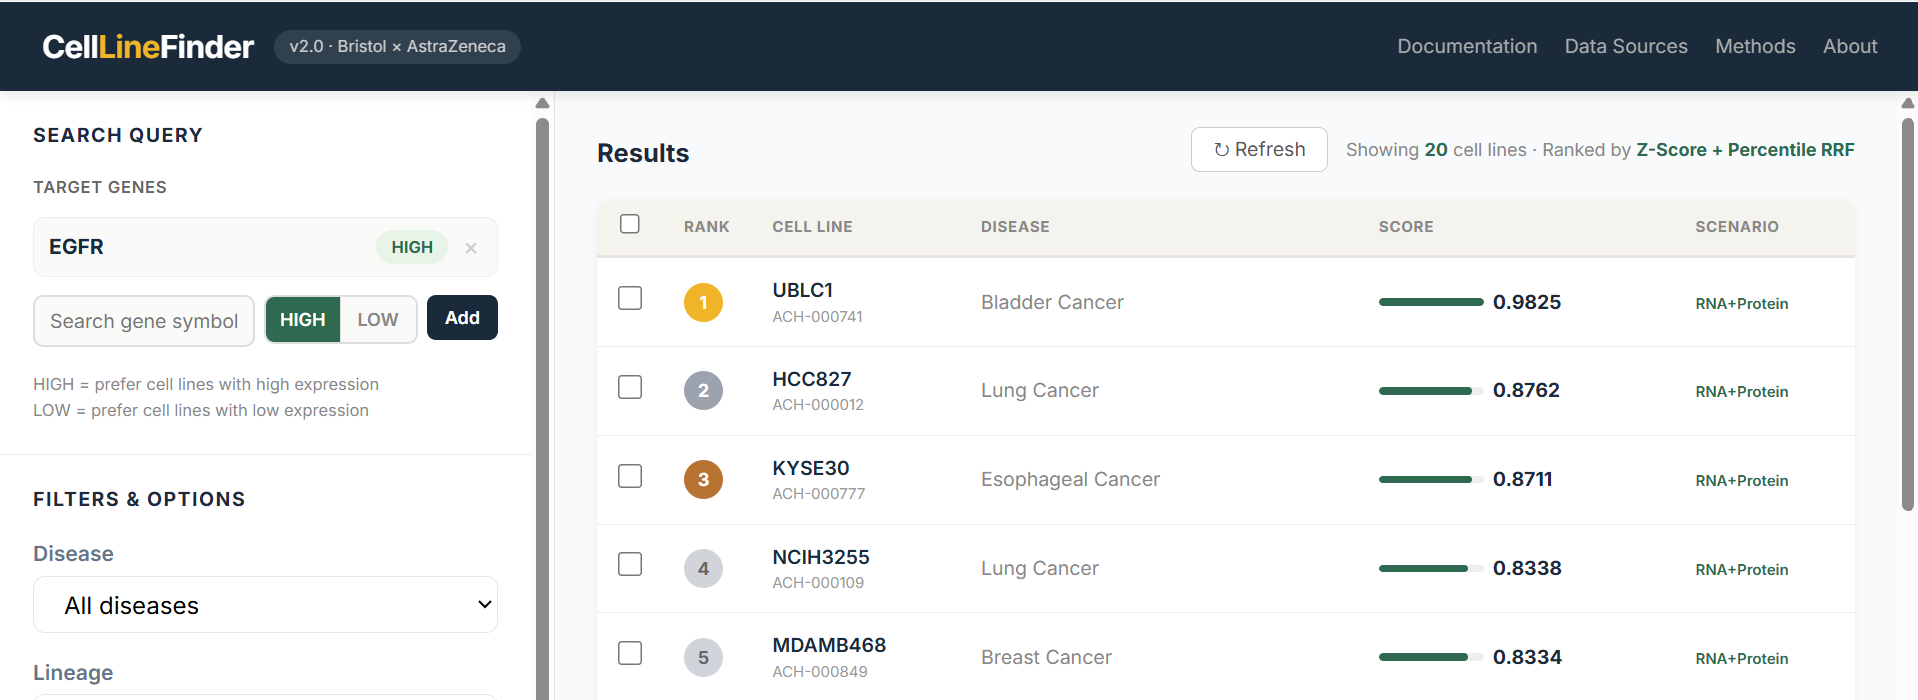
\includegraphics[width=\textwidth]{figures/egfr_base_case.png}
\caption{Full query configuration and ranked results for the base case query (EGFR, HIGH, no filters).}
\label{app:egfr-basecase}
\end{figure}

\begin{figure}[h]
\centering
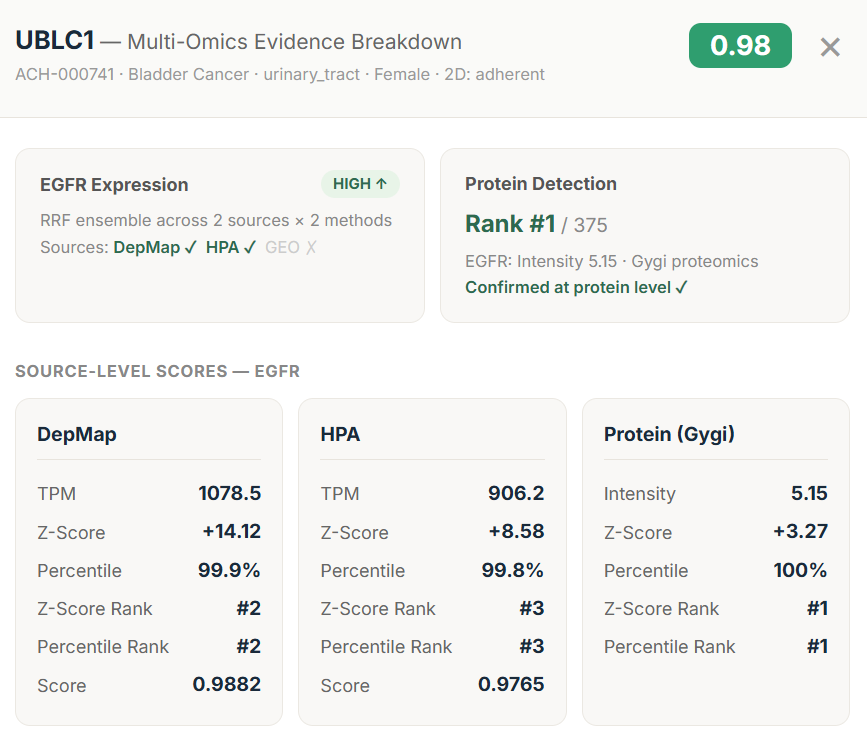
\includegraphics[width=\textwidth]{figures/ublc1_evidence_breakdown.png}
\caption{Multi-omics evidence breakdown panel for UBLC1 (EGFR).}
\label{app:ublc1-breakdown}
\end{figure}


\begin{figure}[t]
\centering
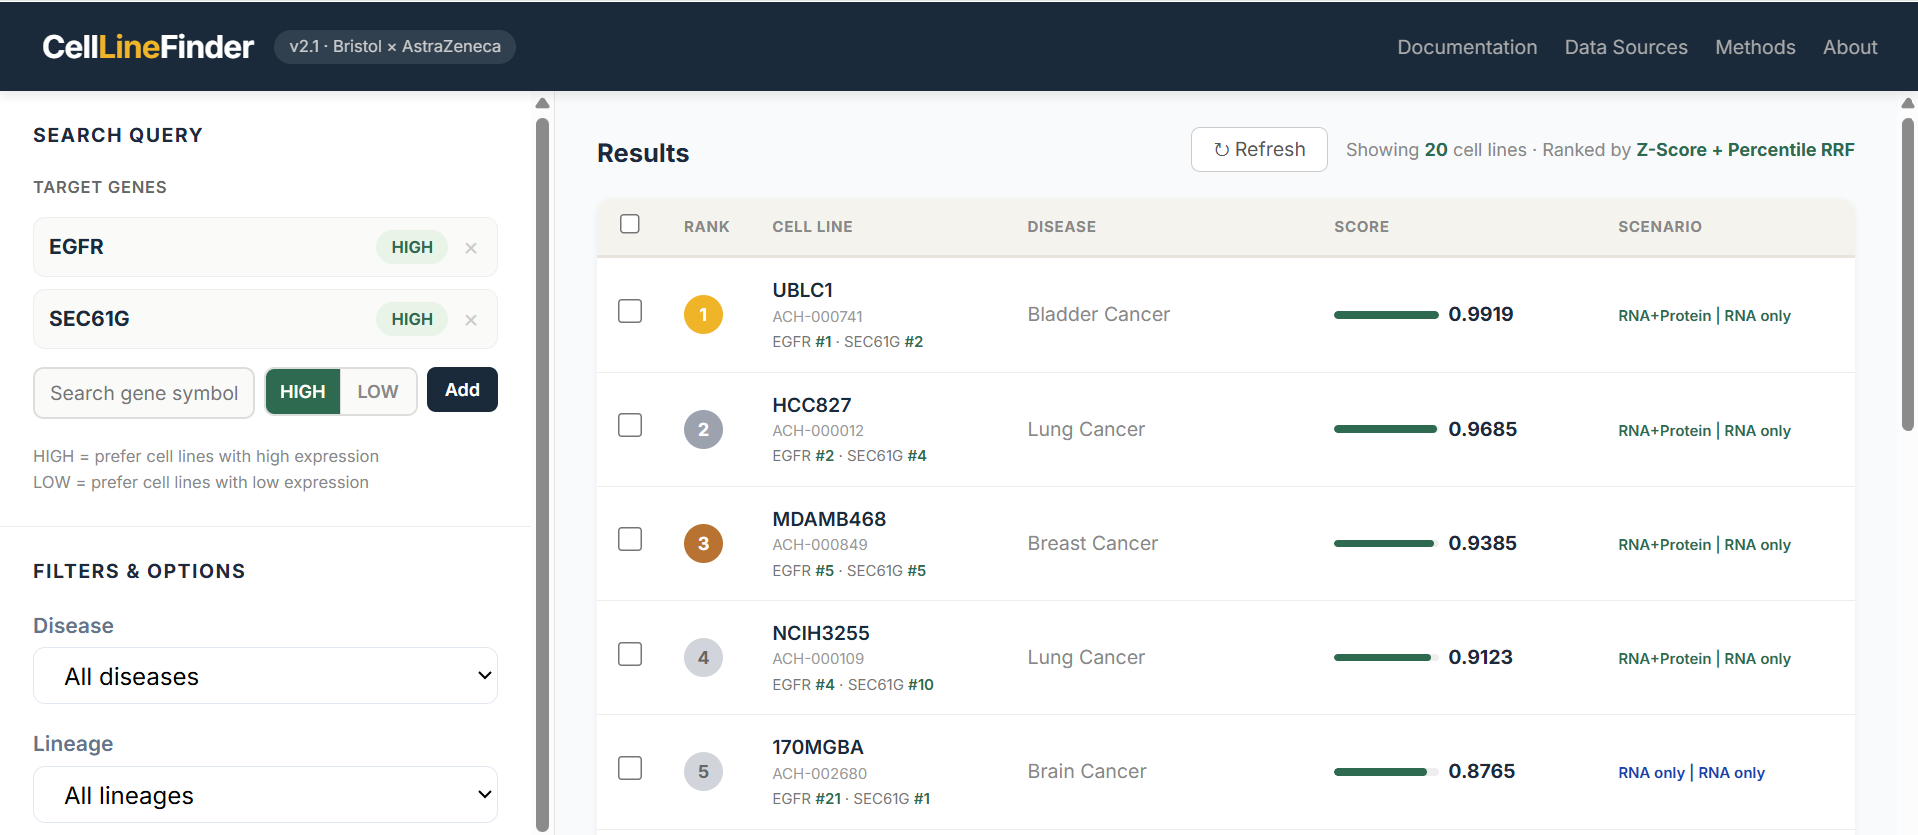
\includegraphics[width=\textwidth]{figures/multigene_no_filter_full.png}
\caption{Full ranked results (top 5) for EGFR + SEC61G (both HIGH), no filters applied.}
\label{app:multigene-full}
\end{figure}
\begin{figure}[h]
\centering
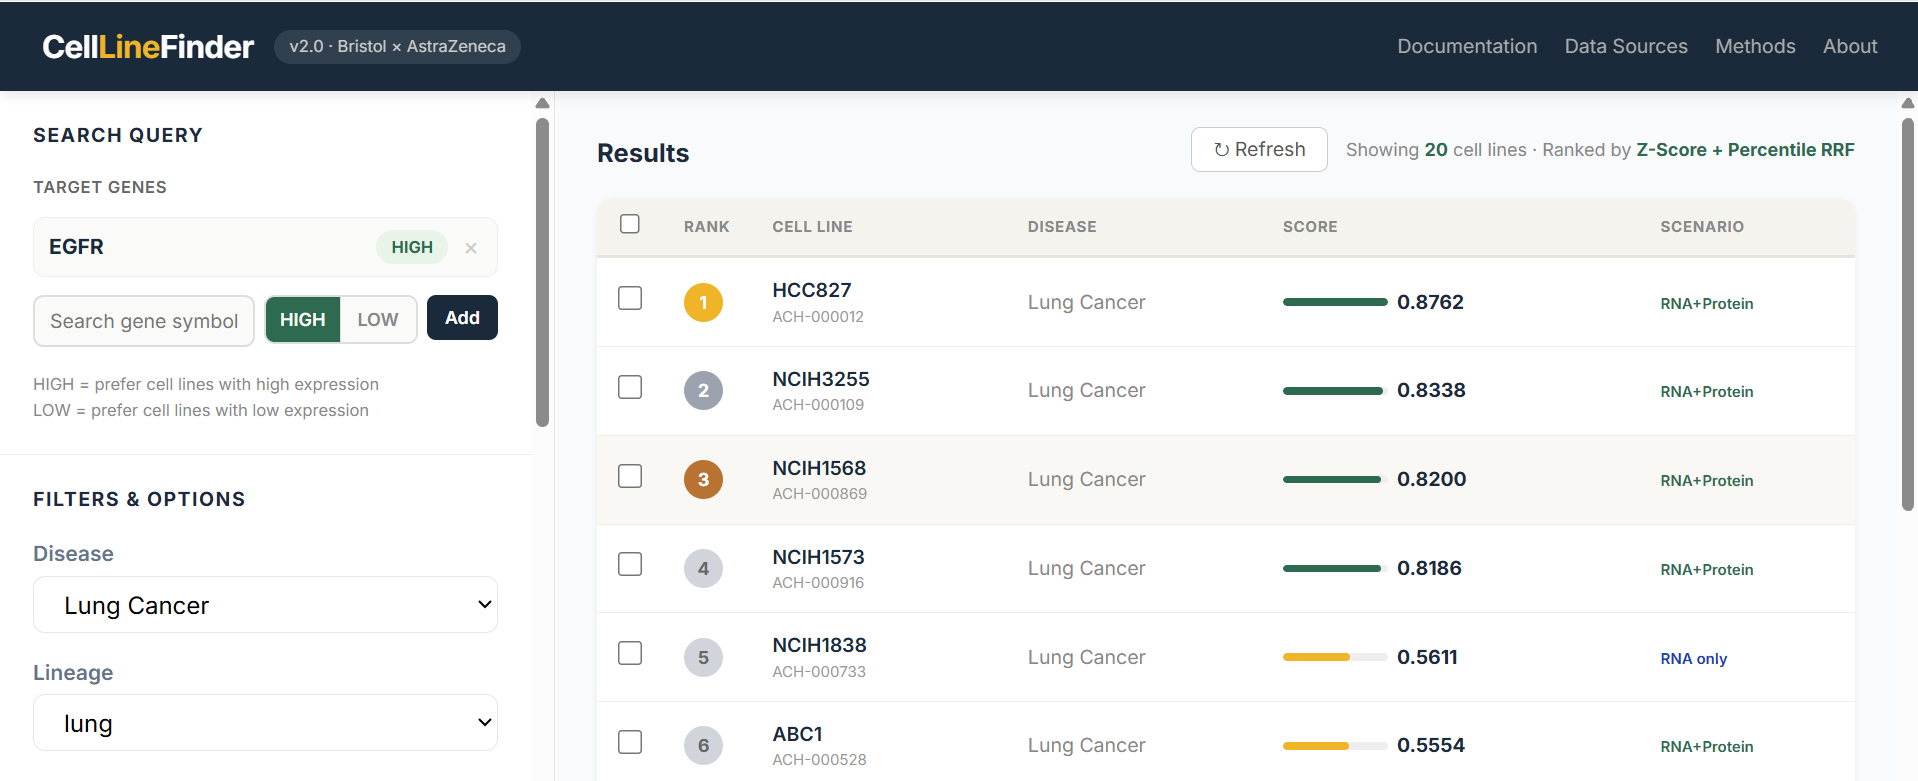
\includegraphics[width=\textwidth]{figures/egfr_lung_filter.png}
\caption{Full query configuration and ranked results for EGFR (HIGH) filtered to Lung Cancer disease and lung lineage.}
\label{app:egfr-lung-filter}
\end{figure}

\begin{figure}[h]
\centering
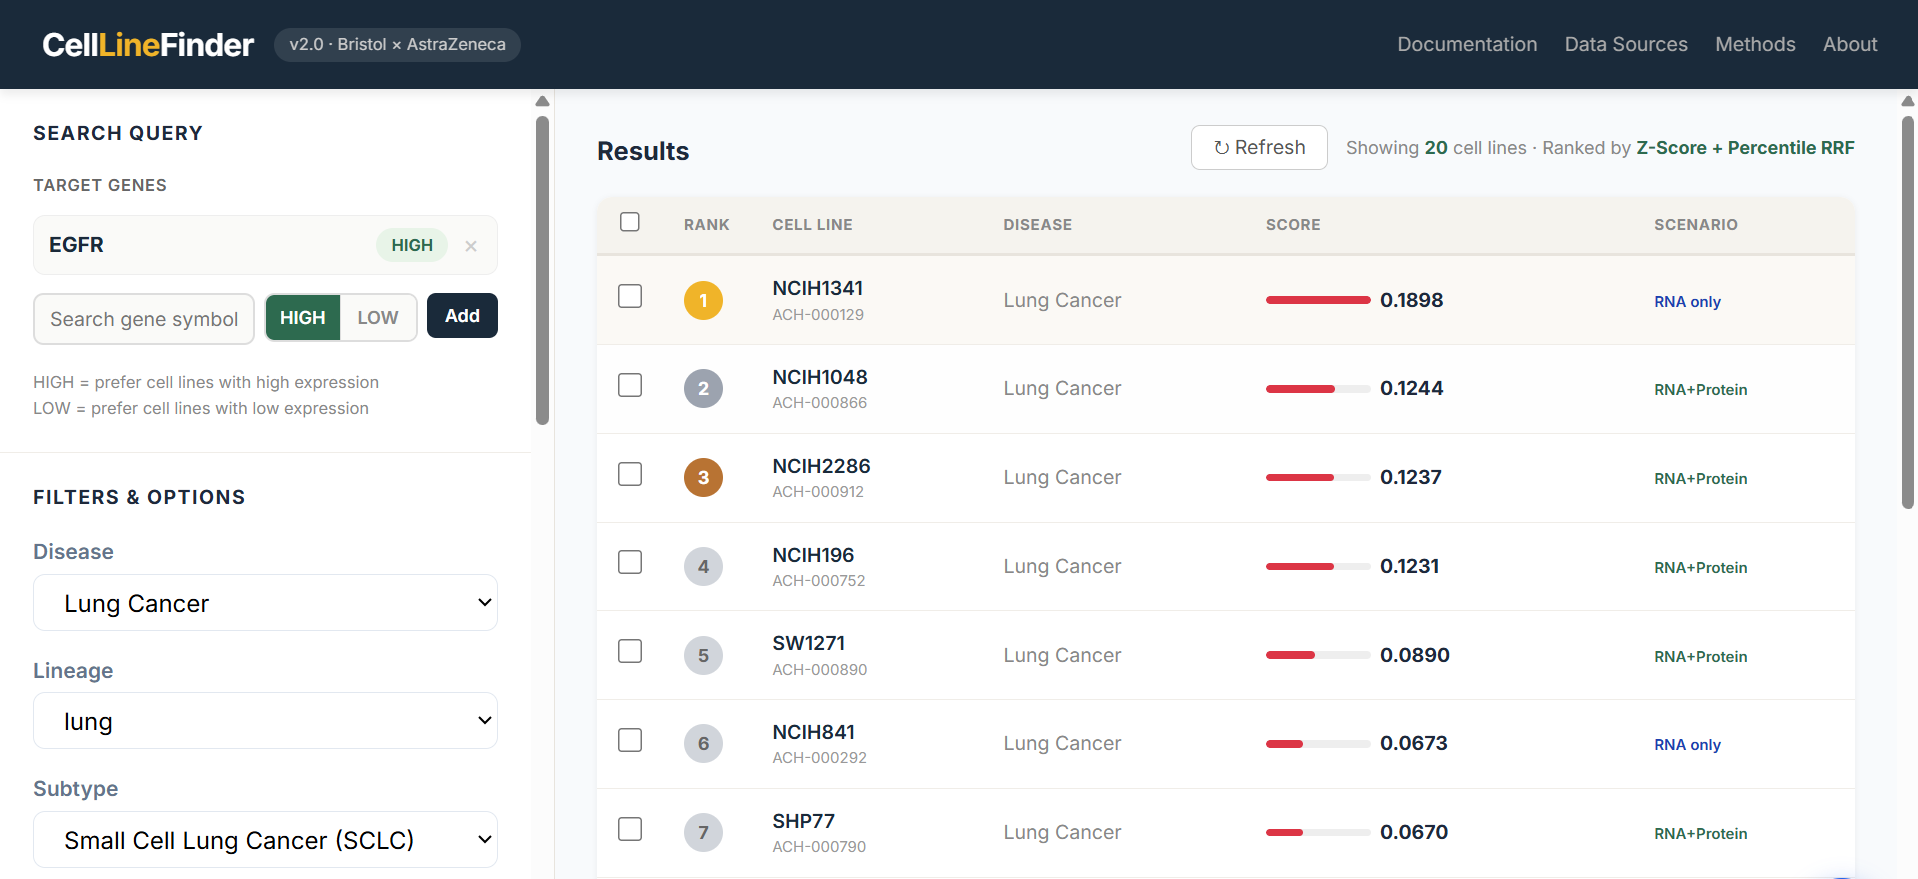
\includegraphics[width=\textwidth]{figures/egfr_sclc_filter.png}
\caption{Full query configuration and ranked results for EGFR (HIGH) filtered to Lung Cancer disease, lung lineage, and SCLC subtype.}
\label{app:egfr-sclc-filter}
\end{figure}

\begin{figure}[h]
\centering
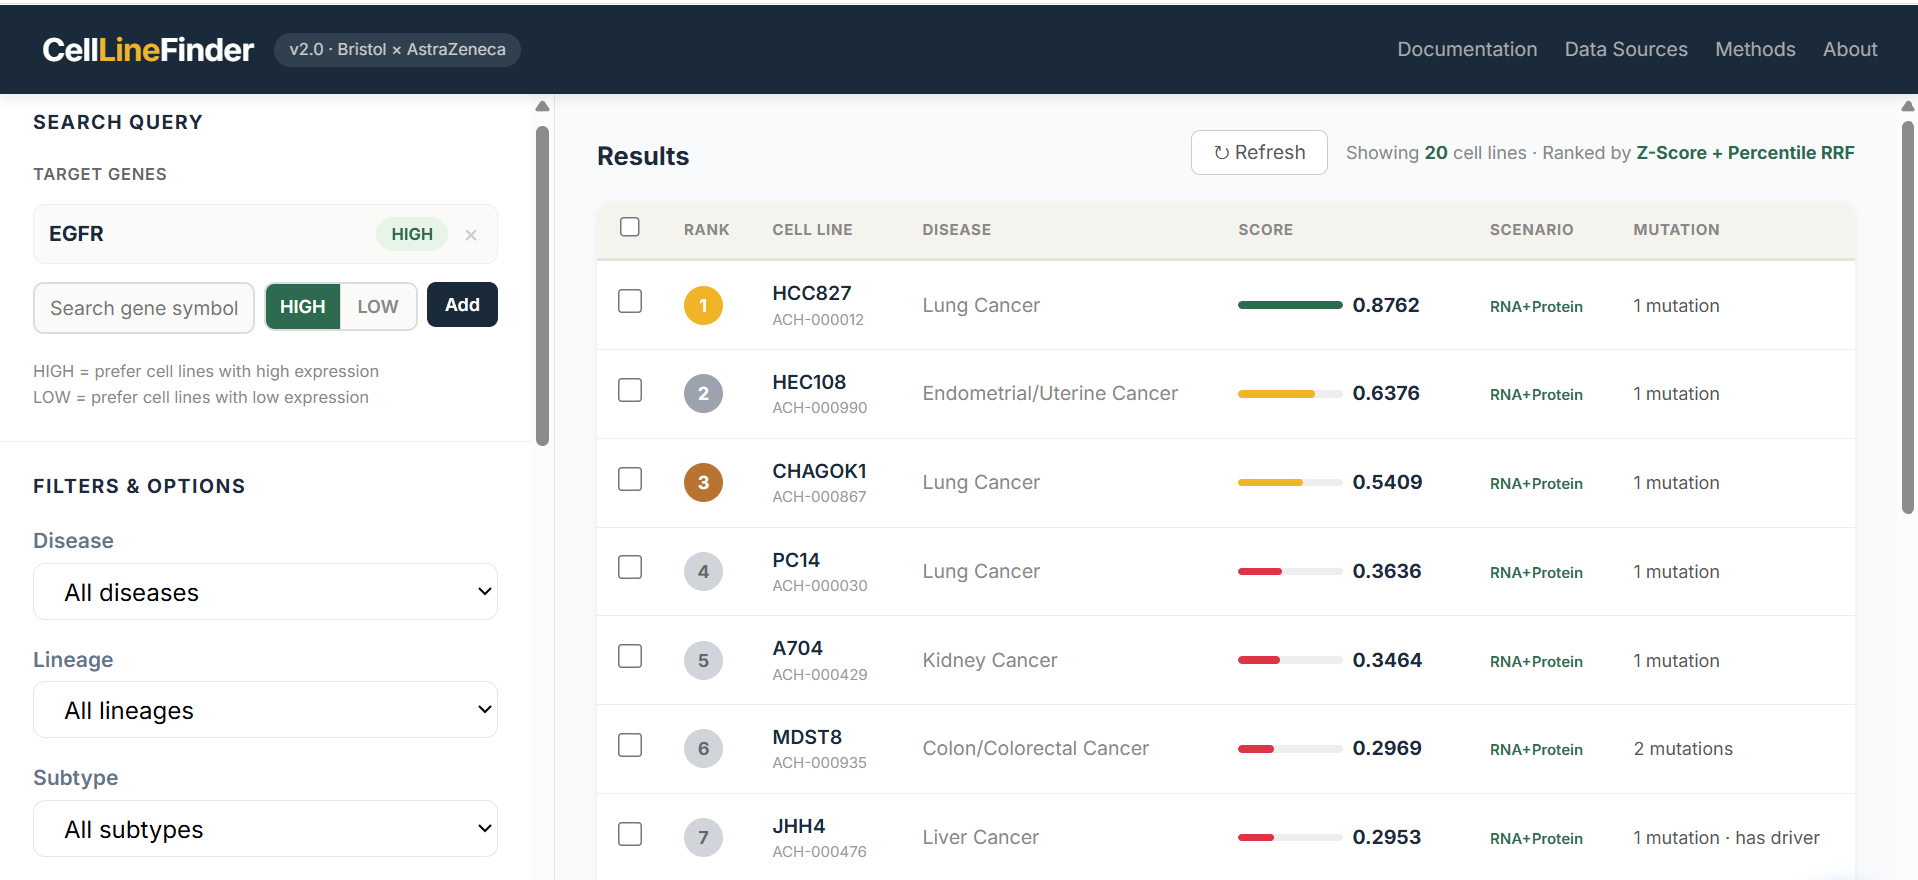
\includegraphics[width=\textwidth]{figures/egfr_mutation_filter.png}
\caption{Full query configuration and ranked results for EGFR (HIGH) with mutation filter set to Include.}
\label{app:egfr-mutation-filter}
\end{figure}

\begin{figure}[h]
\centering
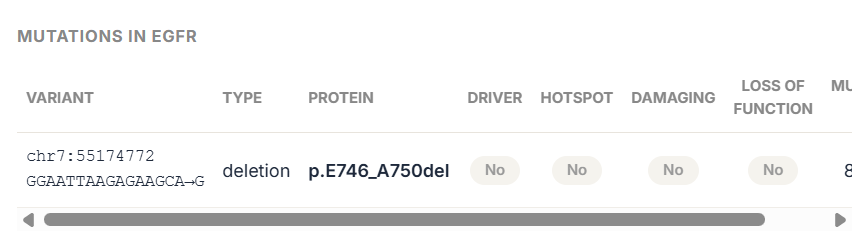
\includegraphics[width=\textwidth]{figures/hcc827_mutation_detail.png}
\caption{Mutation detail panel for HCC827 (EGFR), showing the recorded driver/hotspot/damaging annotations.}
\label{app:hcc827-mutation-detail}
\end{figure}

\begin{figure}[h]
\centering
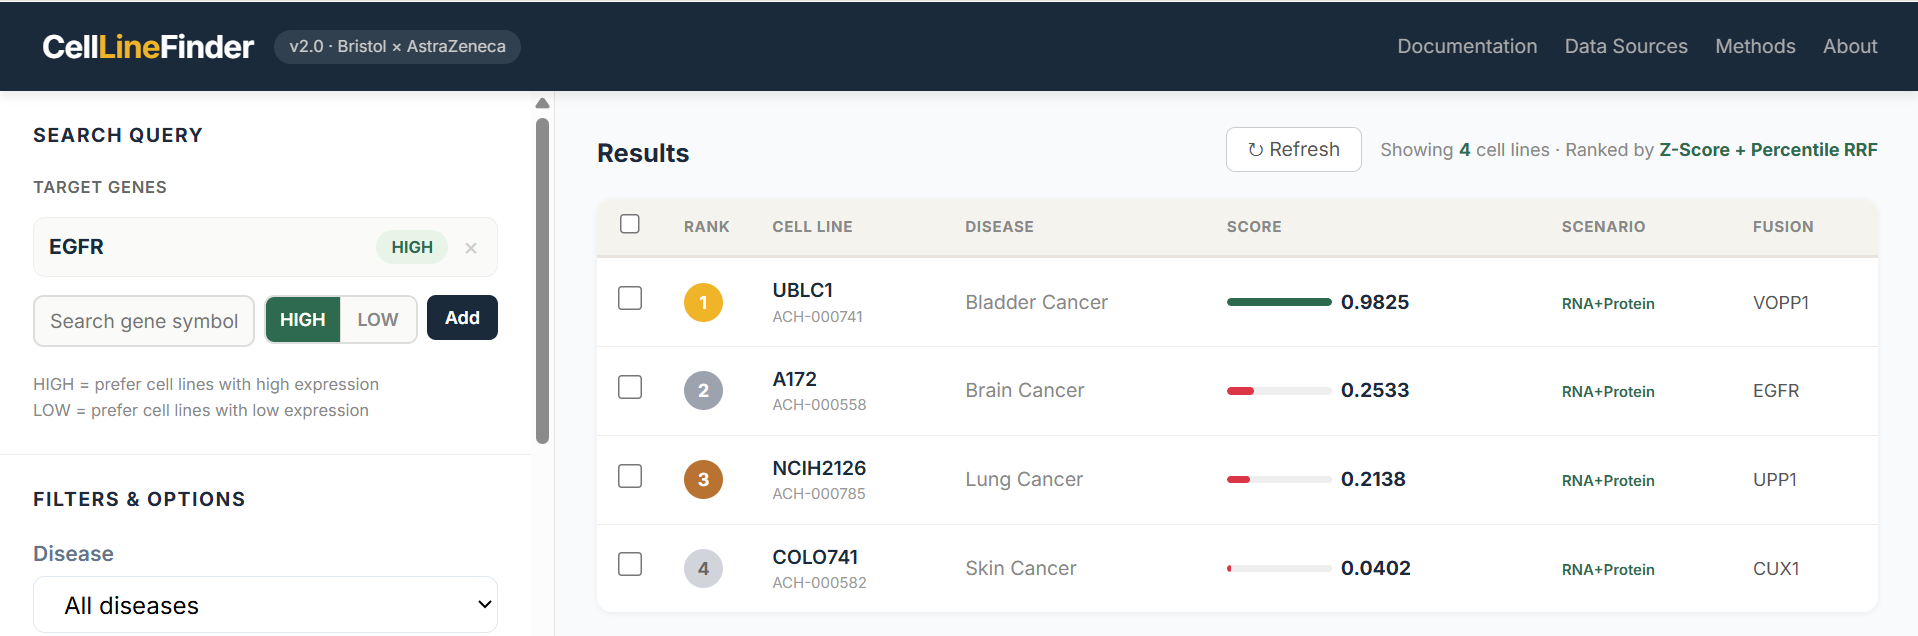
\includegraphics[width=\textwidth]{figures/egfr_fusion_filter.png}
\caption{Full query configuration and ranked results for EGFR (HIGH) with fusion filter set to Include.}
\label{app:egfr-fusion-filter}
\end{figure}

\begin{figure}[h]
\centering
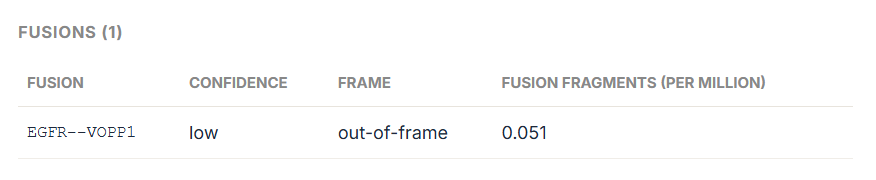
\includegraphics[width=\textwidth]{figures/ublc1_fusion_detail.png}
\caption{Fusion detail panel for UBLC1, showing the EGFR--VOPP1 fusion call.}
\label{app:ublc1-fusion-detail}
\end{figure}

\begin{figure}[h]
\centering
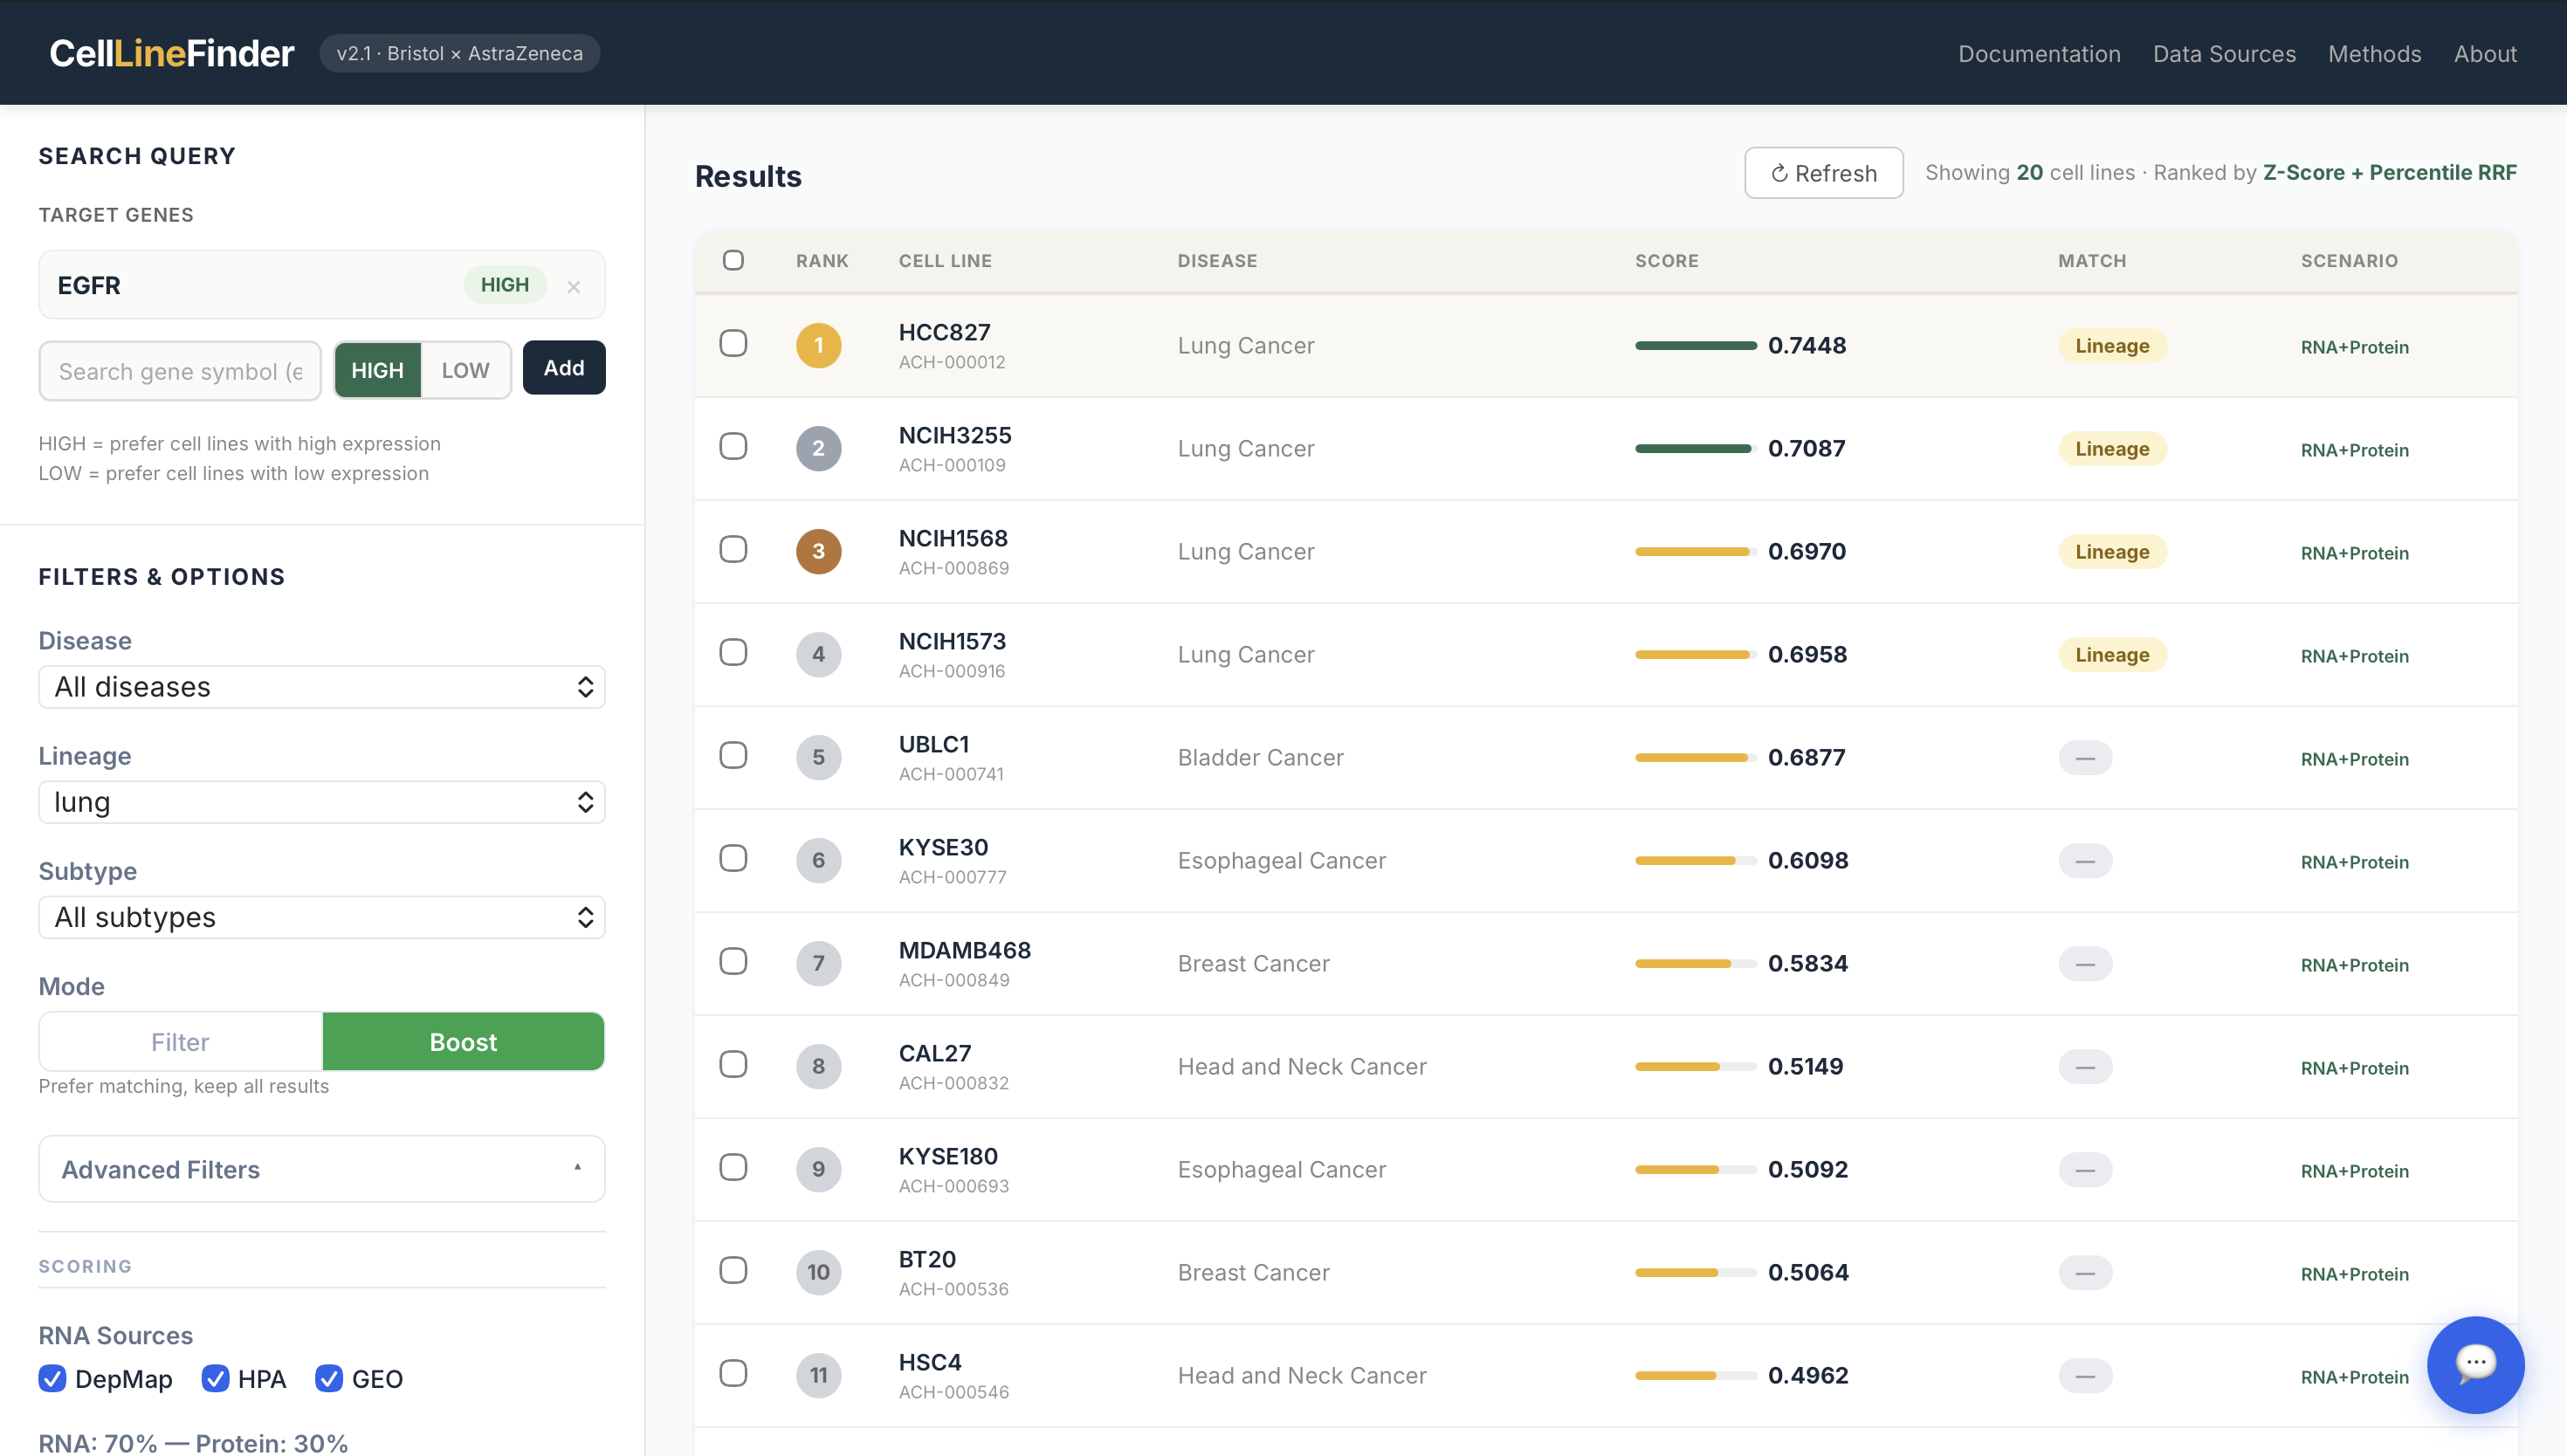
\includegraphics[width=\textwidth]{figures/A10-disease-indication.png}
\caption{Full query configuration and ranked results for EGFR (HIGH) with \texttt{target\_lineage} set to \emph{lung} and soft boost enabled.}
\label{app:A10}
\end{figure}

\begin{figure}[h]
\centering
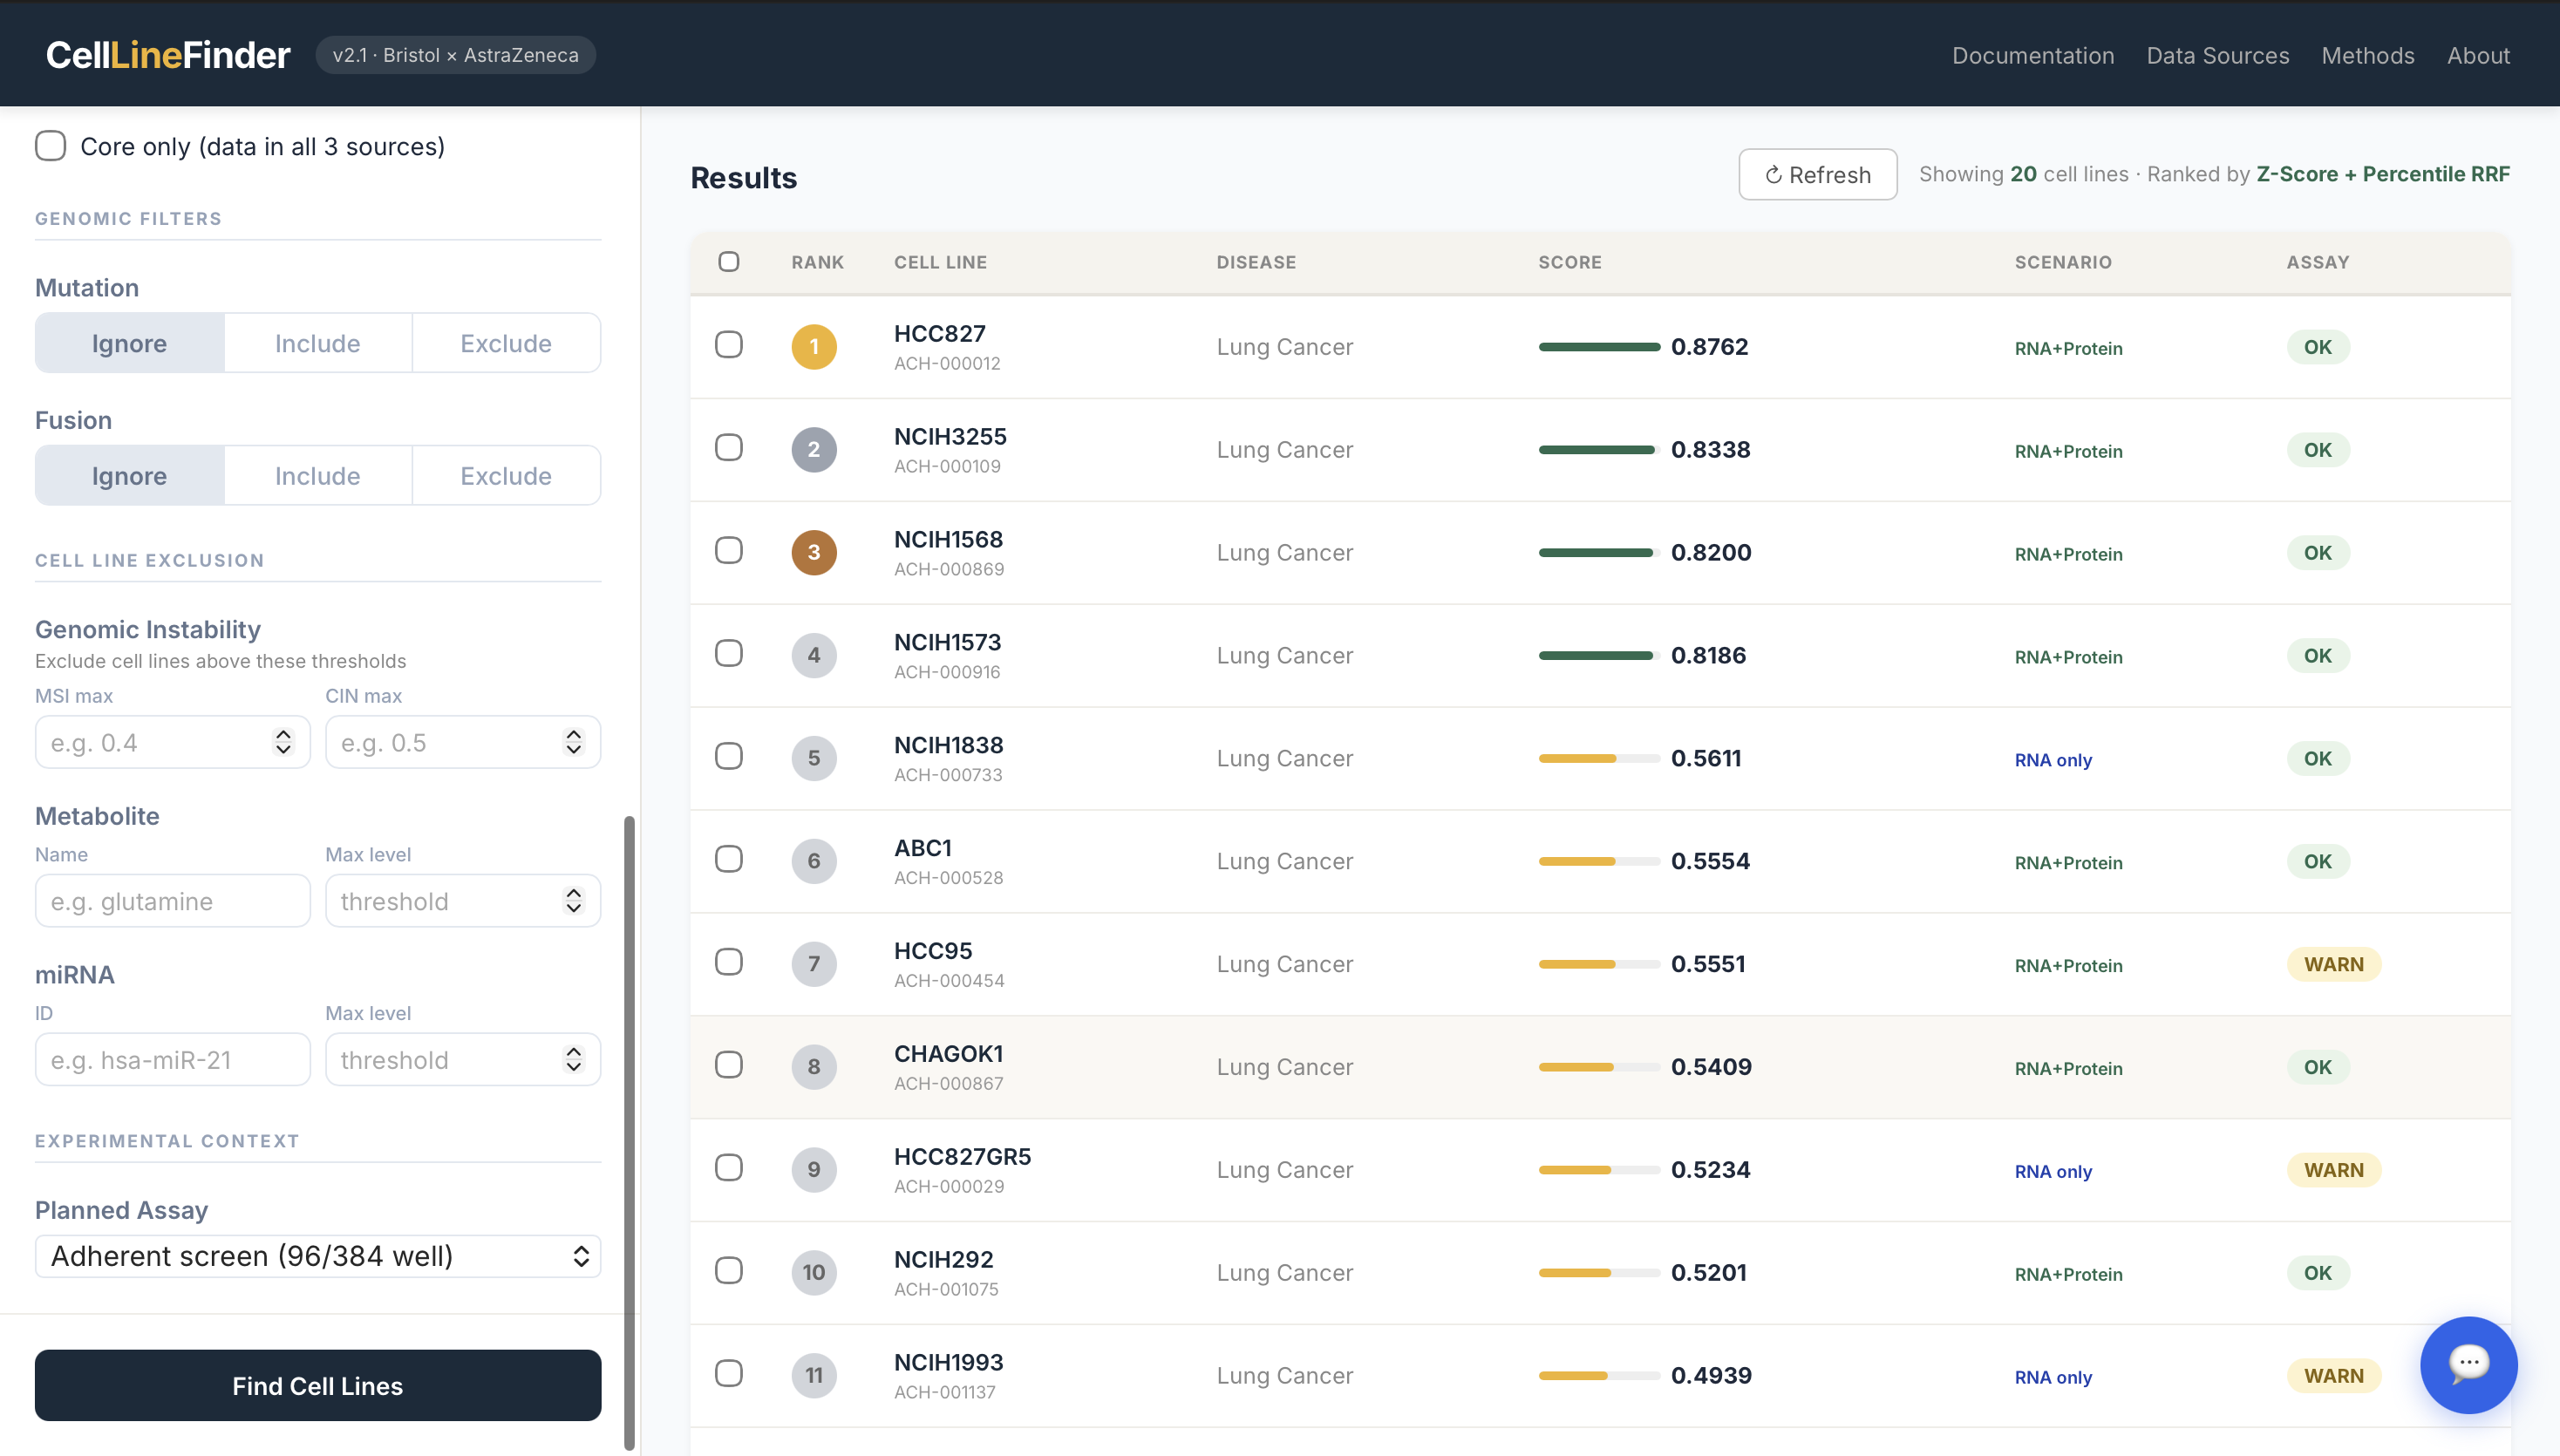
\includegraphics[width=\textwidth]{figures/A11-assay-annotation.png}
\caption{Full query configuration and ranked results for EGFR (HIGH), Lung Cancer + lung filtered, with \texttt{assay\_type} set to \emph{adherent\_screen}.}
\label{app:A11}
\end{figure}

% =============================================================================
\chapter{Supporting Figure for the Similarity Evaluation}
\label{app:similarity}

\begin{figure}[h]
\centering
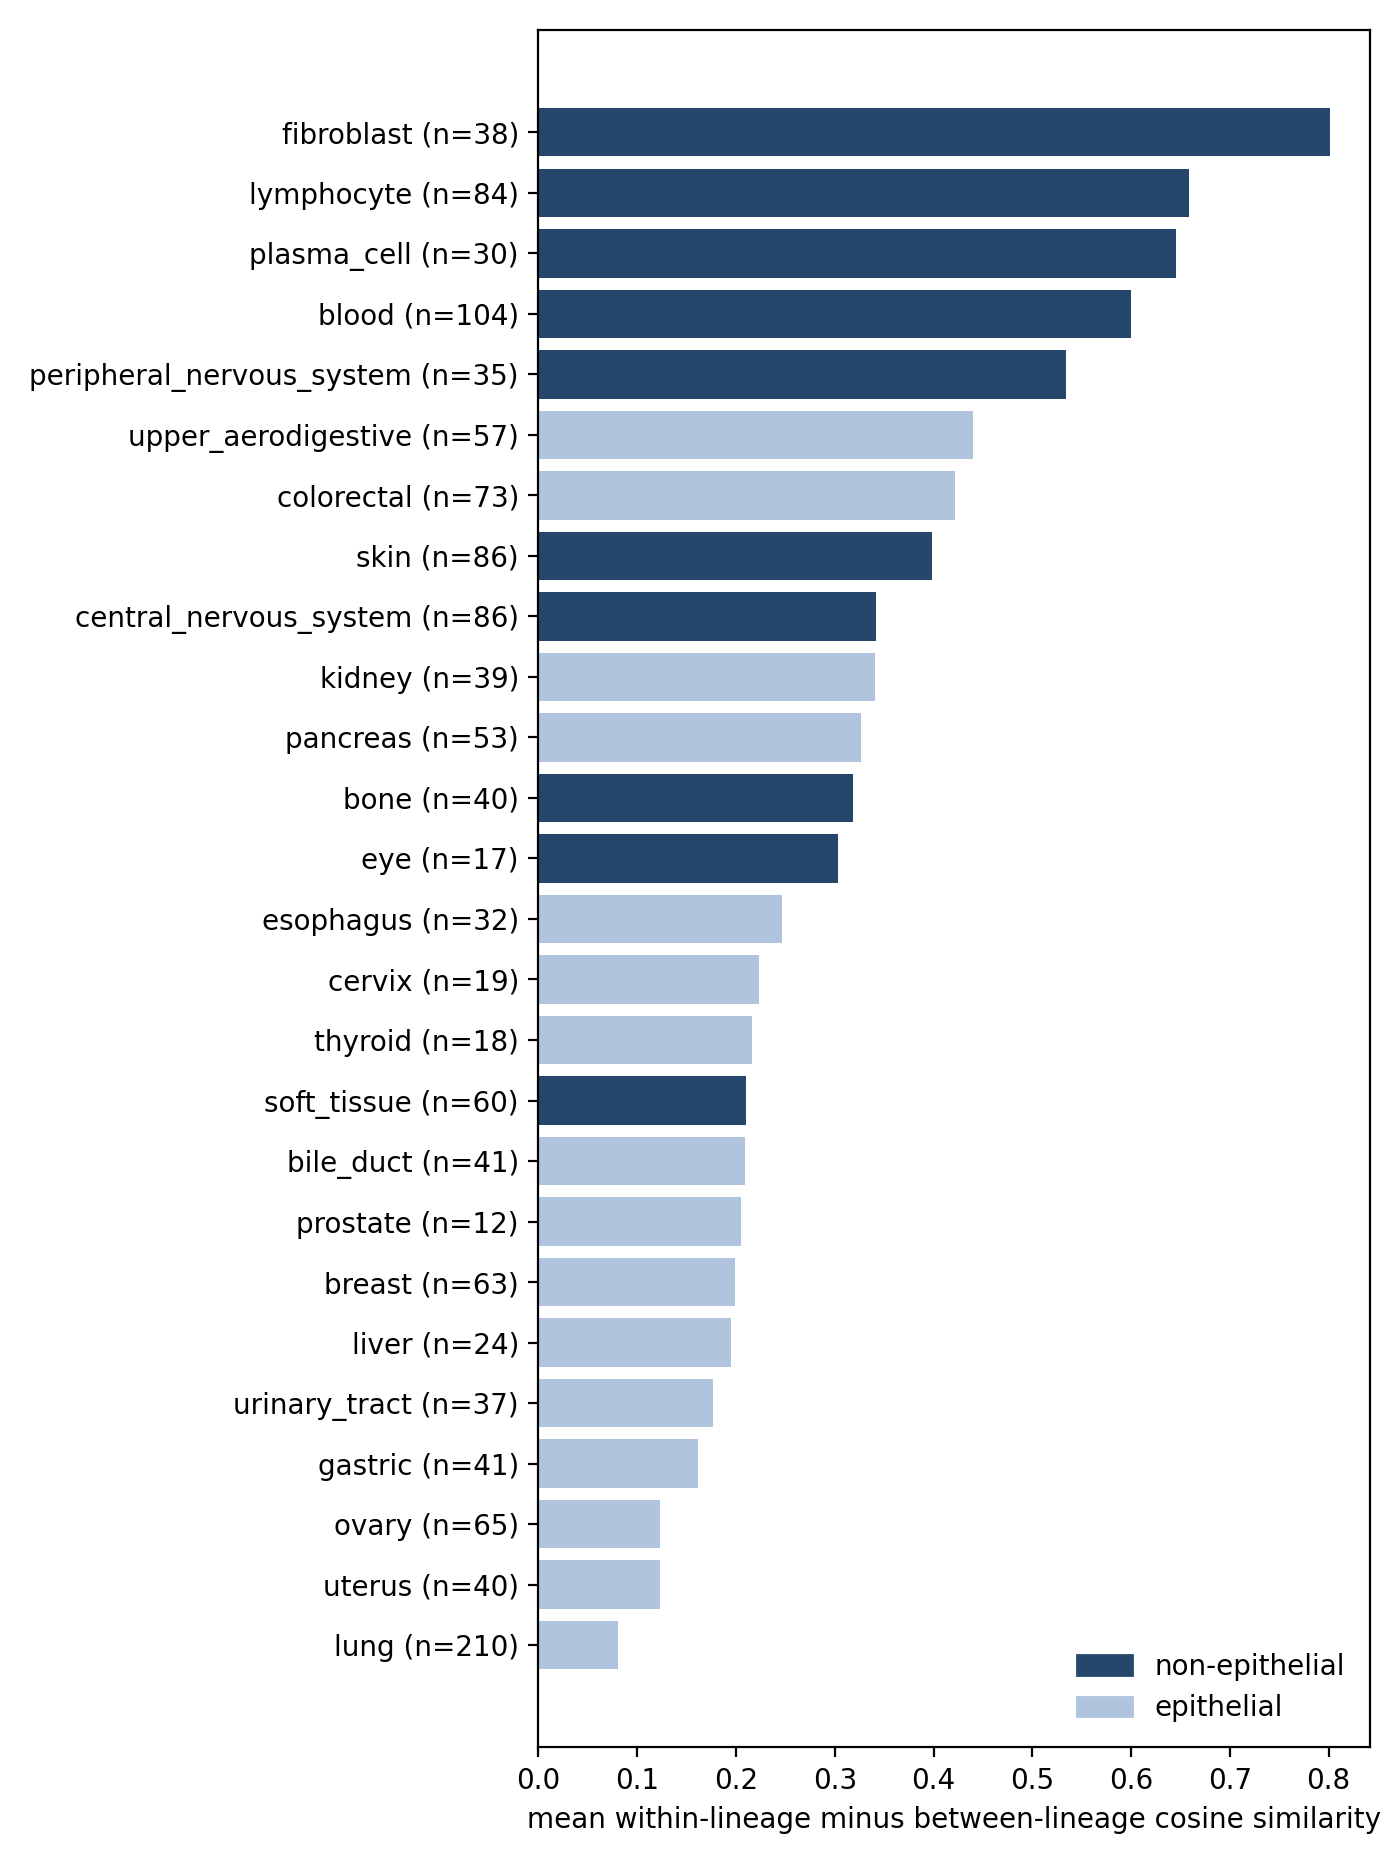
\includegraphics[width=0.7\textwidth]{figures/lineage_separation.png}
\caption{Mean within-lineage minus between-lineage cosine similarity, for the 26 lineages with at least five cell lines. Non-epithelial lineages separate more cleanly than solid epithelial ones.}
\label{app:lineage-separation}
\end{figure}
% =============================================================================
\chapter{Source Code and Deployment}
\label{app:code}

The full source code for CellLineFinder, including the FastAPI backend, 
React frontend, data harmonisation notebooks, ranking algorithm, and 
evaluation scripts referenced throughout Chapter~\ref{chap:evaluation}, is 
available at:

\begin{center}
\url{https://github.com/NattawasP/SEMTM0044_2025_AYEAR_TEAM34}
\end{center}

\bigskip
\noindent
The deployed platform is publicly accessible at:

\begin{center}
\url{https://celllinefinder.com/}
\end{center}

\end{document}
